% !TEX root =  ../../../thesis.tex
%%%%%%%%%%%%%%%%%%%%%%%%%%%%%%%%%%%%%%%%%%
\begin{figure}
    \centering
    {
    \captionsetup[subfigure]{labelformat=empty}
    \subfloat[0.03]{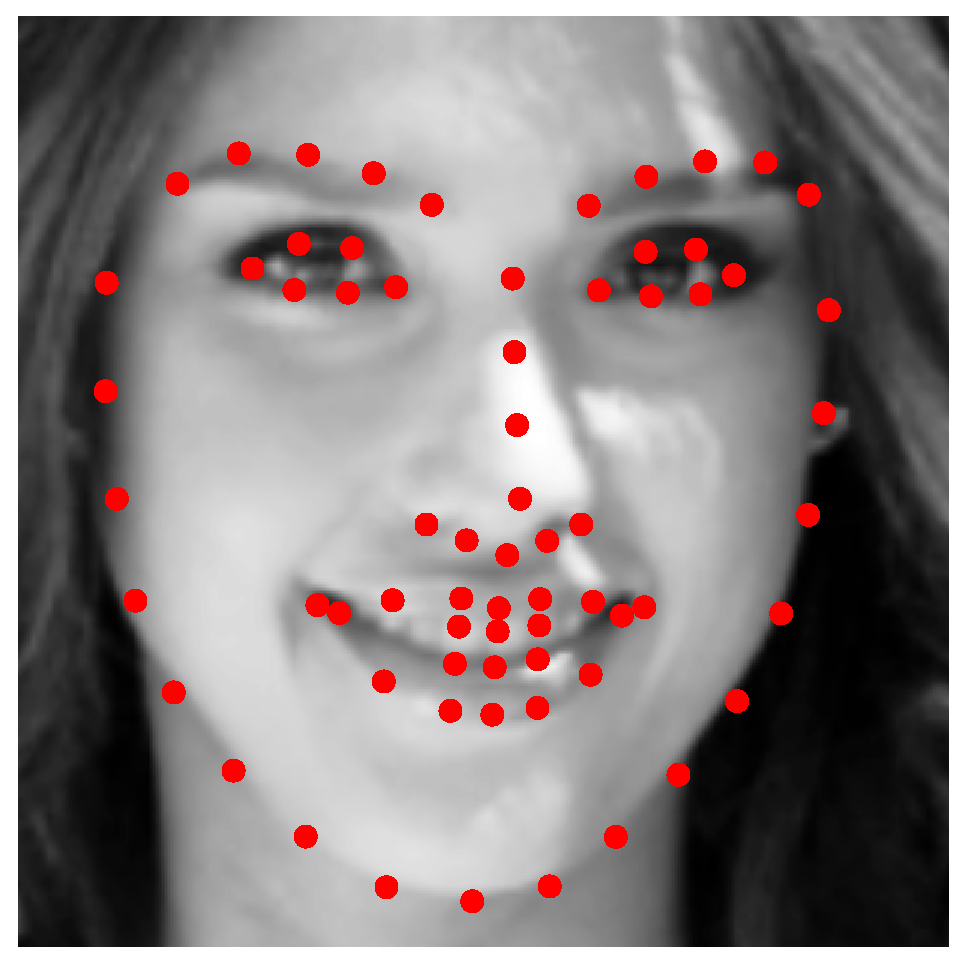
\includegraphics[width=0.22\columnwidth]{figures/acr/errors_examples/points68_err3_im301.eps}}
    \subfloat[0.04]{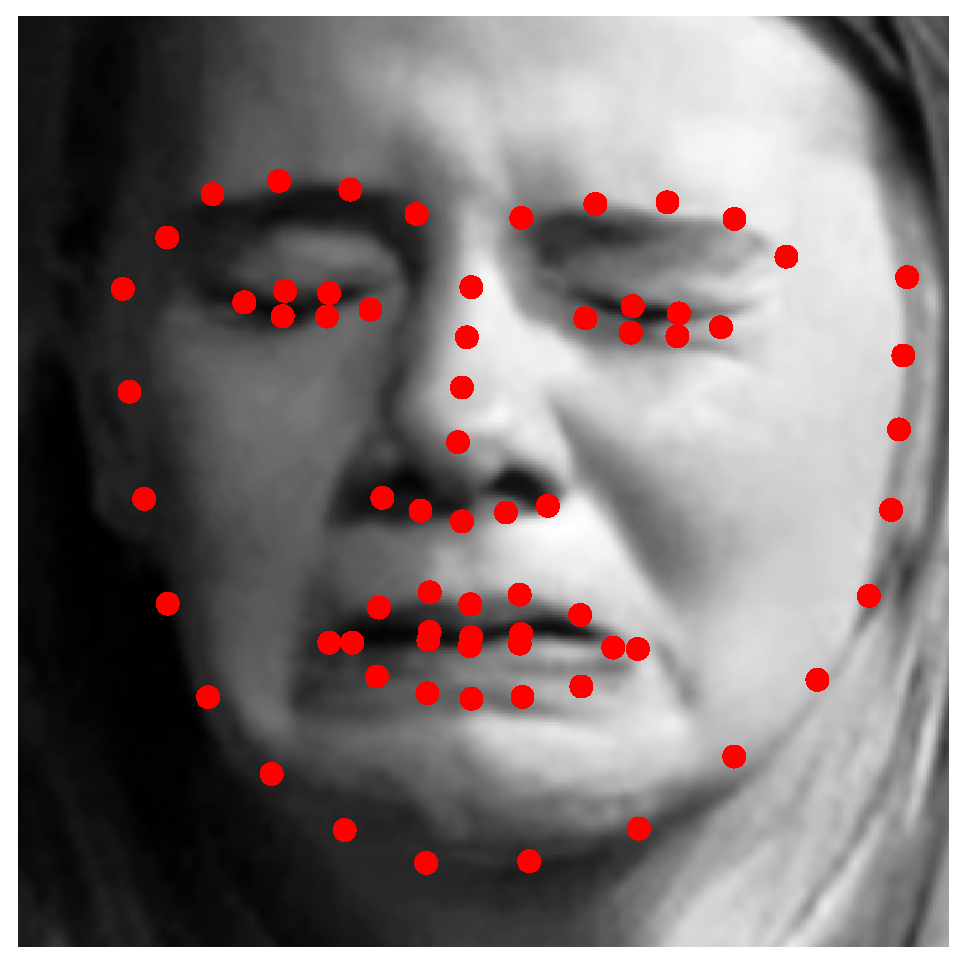
\includegraphics[width=0.22\columnwidth]{figures/acr/errors_examples/points68_err4_im591.eps}}
    \subfloat[0.05]{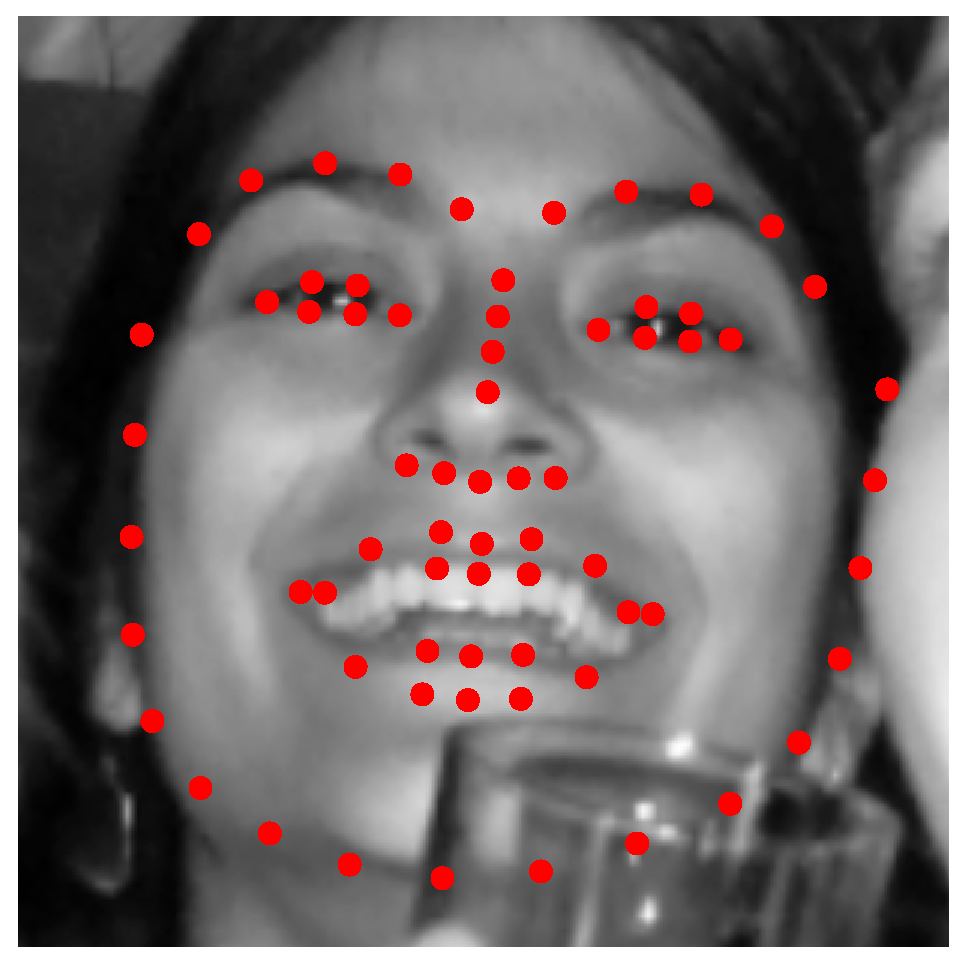
\includegraphics[width=0.22\columnwidth]{figures/acr/errors_examples/points68_err5_im143.eps}}
    \subfloat[0.06]{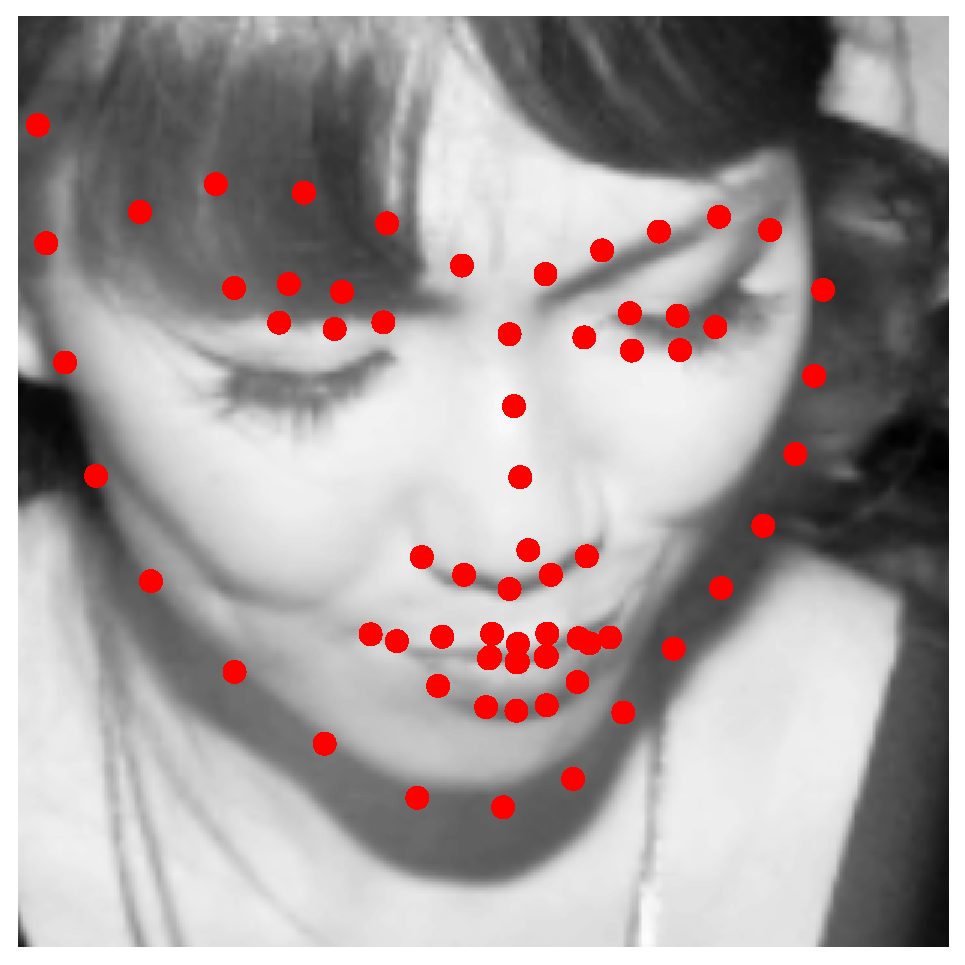
\includegraphics[width=0.22\columnwidth]{figures/acr/errors_examples/points68_err6_im226.eps}}
    \\ \vspace*{-0.3cm}
    \subfloat[0.03]{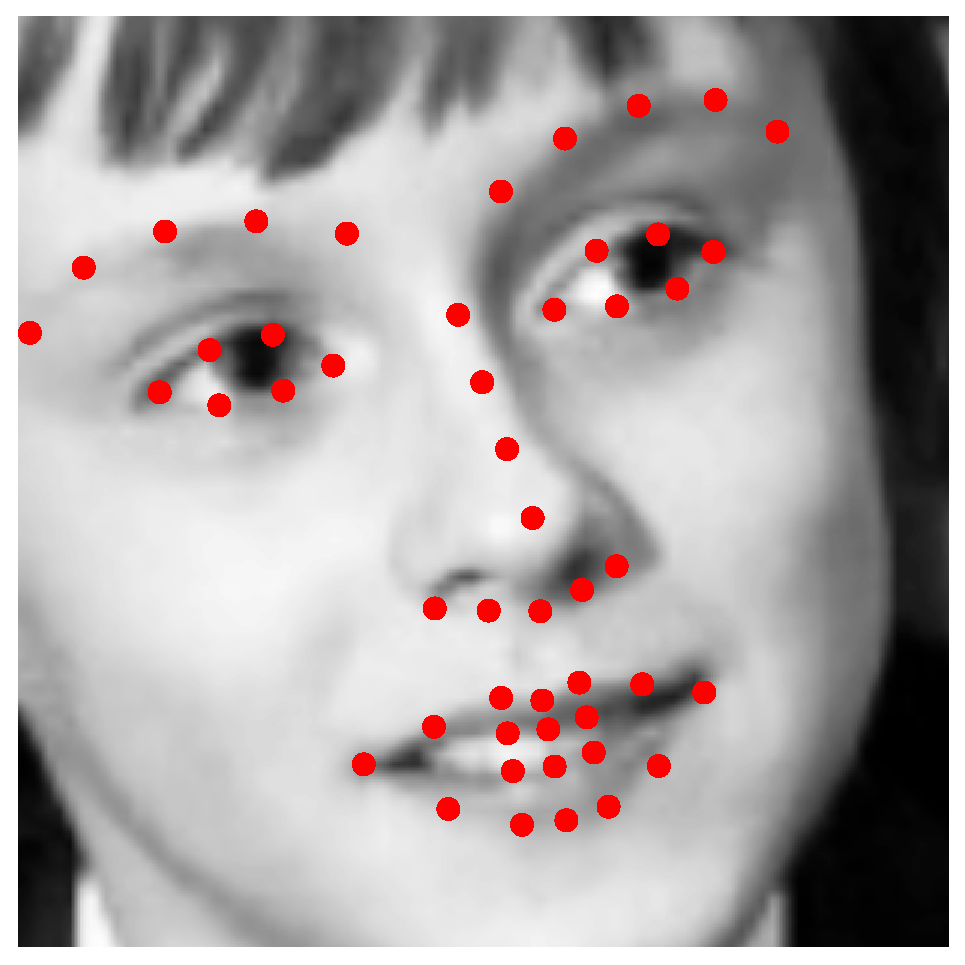
\includegraphics[width=0.22\columnwidth]{figures/acr/errors_examples/points49_err3_im227.eps}}
    \subfloat[0.04]{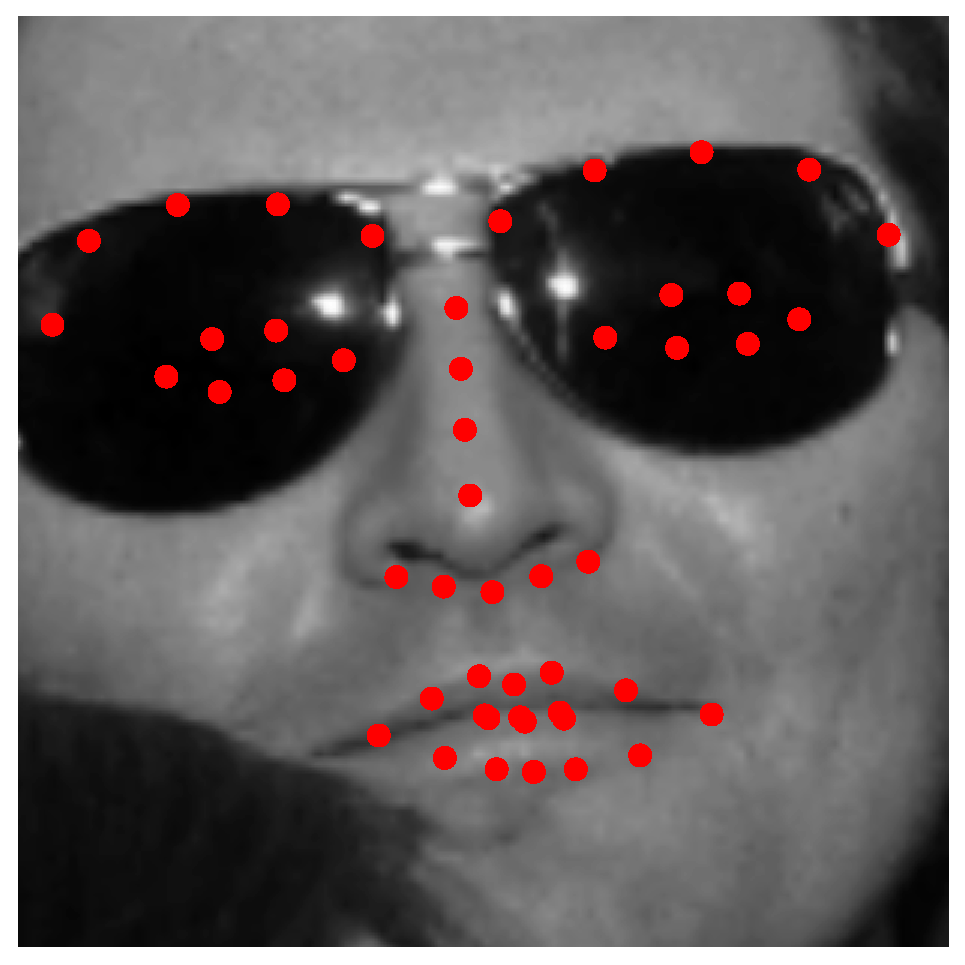
\includegraphics[width=0.22\columnwidth]{figures/acr/errors_examples/points49_err4_im487.eps}}
    \subfloat[0.05]{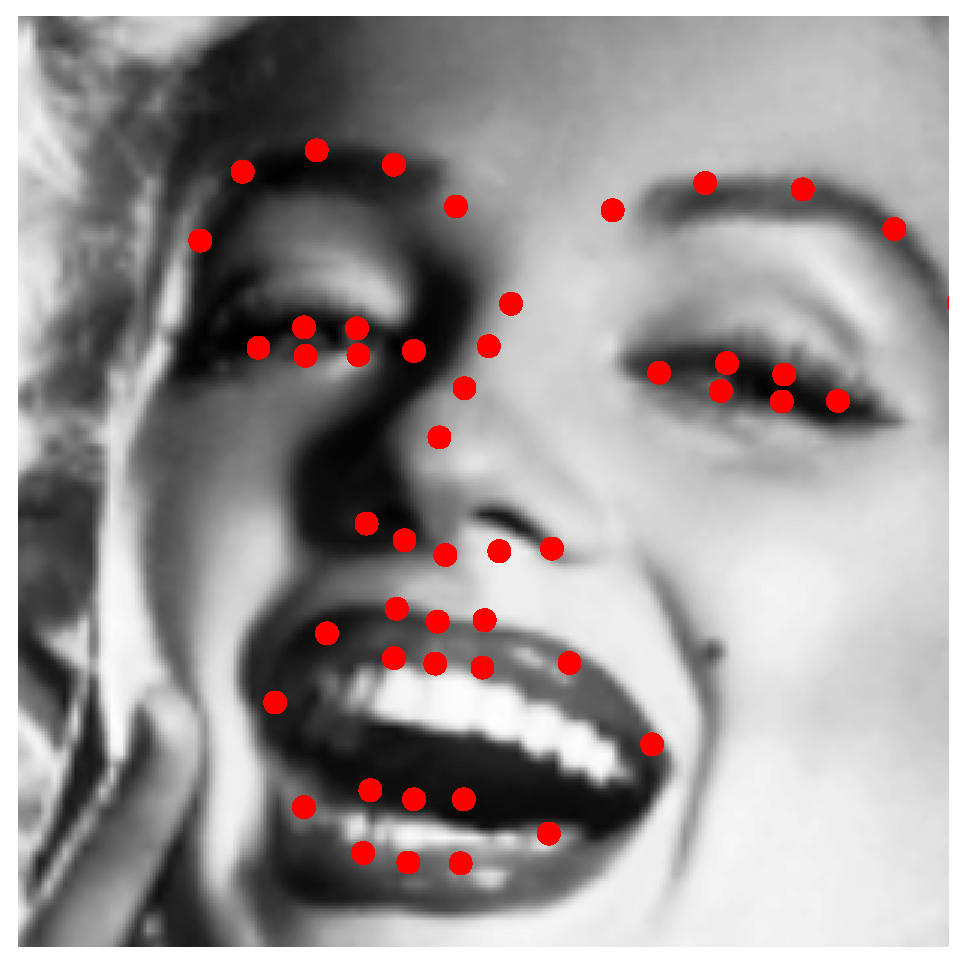
\includegraphics[width=0.22\columnwidth]{figures/acr/errors_examples/points49_err5_im82.eps}}
    \subfloat[0.06]{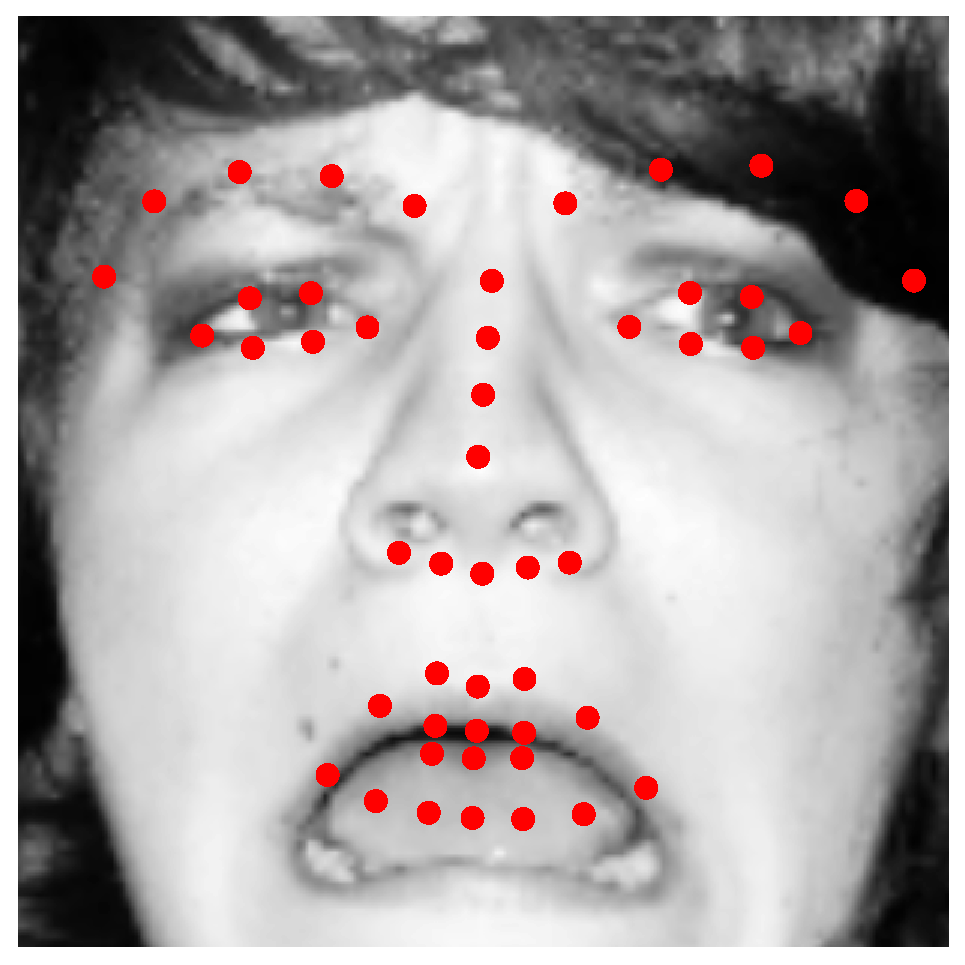
\includegraphics[width=0.22\columnwidth]{figures/acr/errors_examples/points49_err6_im569.eps}}
    }
    \caption{Representative examples of increasing normalised errors. (\emph{top}) 68-points. (\emph{bottom}) 49-points.}
\label{fig:error_examples}
\end{figure}
%%%%%%%%%%%%%%%%%%%%%%%%%%%%%%%%%%%%%%%%%%
%%%%%%%%%%%%%%%%%%%%%%%%%%%%%%%%%%%%%%%%%%%%%%%%%%%%%%%%%%%%%%%%%%%%%%
\section{Experimental Results}\label{sec:acr:experiments}

\paragraph{Evaluation Protocol} To maintain consistency with the results
of the original 300-W competition, we report Cumulative Error Distribution
(CED) graphs using the point-to-point error normalized by the interocular
distance defined by the outer eye corners. The mean error often reported
in recent works~\cite{ren2014face,zhu2015face} is highly biased by
alignments that completely fail. Therefore, we believe that the failure rate
as shown in~\cite{burgos2013robust} is a much more informative error metric.
To complement the failure rate, we propose the area under the curve (AUC),
which enables simpler comparison of CED curves that are otherwise difficult
to compare. We fix a maximum error that we believe represents a failed fitting,
and thus the higher the AUC, the more fittings are concentrated within
this acceptable fitting area. In all experiments, CED curves and AUC errors
are reported up to $0.06$. Examples of different errors are
given in Figure~\ref{fig:error_examples}, which shows that $0.06$ represents an
alignment failure.

\paragraph{Implementation Details} The following settings were used for
training ACR. $20$ components were kept for the shape model and $300$ for the
appearance model. After running extended cross-validation experiments, we found
that the best performance is obtained by using a cascade of $14$ levels and
setting $\lambda=[1,~0.75,~0.5,~0.25]$ for the first four and $\lambda=0$ for
the rest.
Intuitively, this means that the regression-based descent directions need to
dominate the optimization on the first few iterations, as they are able to move
towards the correct direction with steps of large magnitude. After that, the
gradient descent steps are sufficient in order to converge to an accurate local
minimum.
The first two were performed on the image at half scale, the rest at full
scale. The patch sizes were
$[(32\times32), (24\times24), (24\times24), (16\times16)]$
for the first four cascades and $(24\times24)$ for the rest. Dense
SIFT~\cite{vedaldi2008vlfeat,lowe1999object} features were used for all
methods. When performing a regression, a ridge parameter of $100$ was used. In
order to increase the size of the training data, we augment it by perturbing
the provided bounding boxes of the 300-W competition with uniform noise of
$0.005$ for scaling and $0.07$ for translation (scaled by the bounding box
size). The same options were used for training the generative model (AAM) and
the discriminative cascaded-regression (SDM).

%%%%%%%%%%%%%%%%%%%%%%%%%%%%%%%%%%%%%%%%%%
\begin{figure}[!t]
  \centering
  \hspace{0.6cm}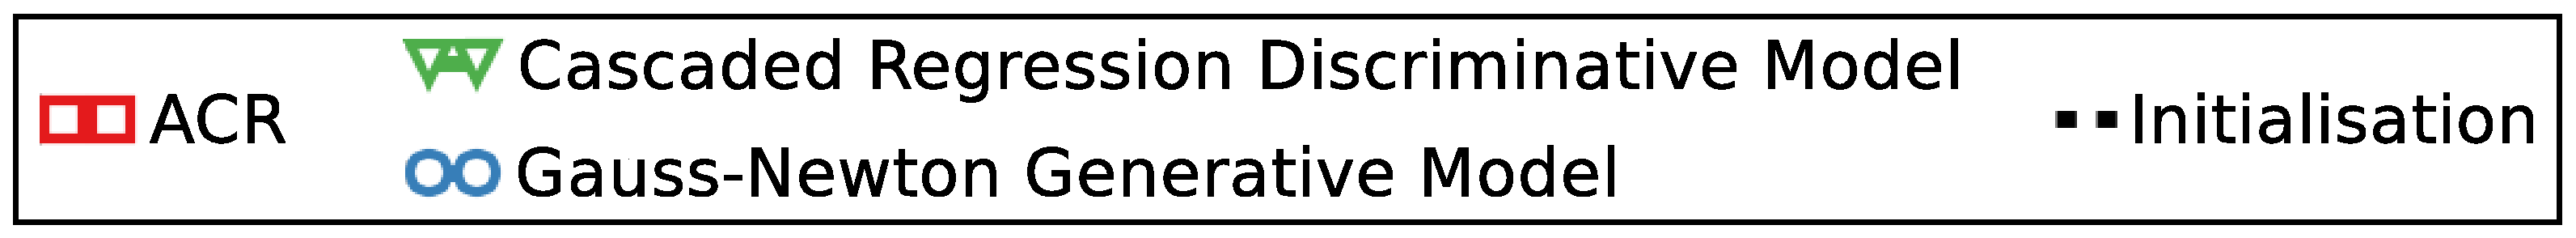
\includegraphics[height=0.90cm]{figures/acr/internal/legend/legend.eps}\\
  \subfloat[68-point error]{
  \includegraphics[width=0.70\linewidth]{figures/acr/internal/accuracy_68_points.eps}}\\
  \subfloat[49-point error]{
  \includegraphics[width=0.70\linewidth]{figures/acr/internal/accuracy_49_points.eps}}
  \caption{ACR, AAM (Gauss-Newton) and SDM (Discriminative), trained identically, tested on the images of AFW\@. Initialization given by the bounding boxes of~\cite{sagonas2013300,sagonas2016faces}.}
  \label{fig:self_eval_afw_ced}
\end{figure}
%%%%%%%%%%%%%%%%%%%%%%%%%%%%%%%%%%%%%%%%%%

%%%%%%%%%%%%%%%%%%%%%%%%%%%%%%%%%%%%%%%%%%
\begin{figure}[!t]
  \centering
  \hspace{1.0cm}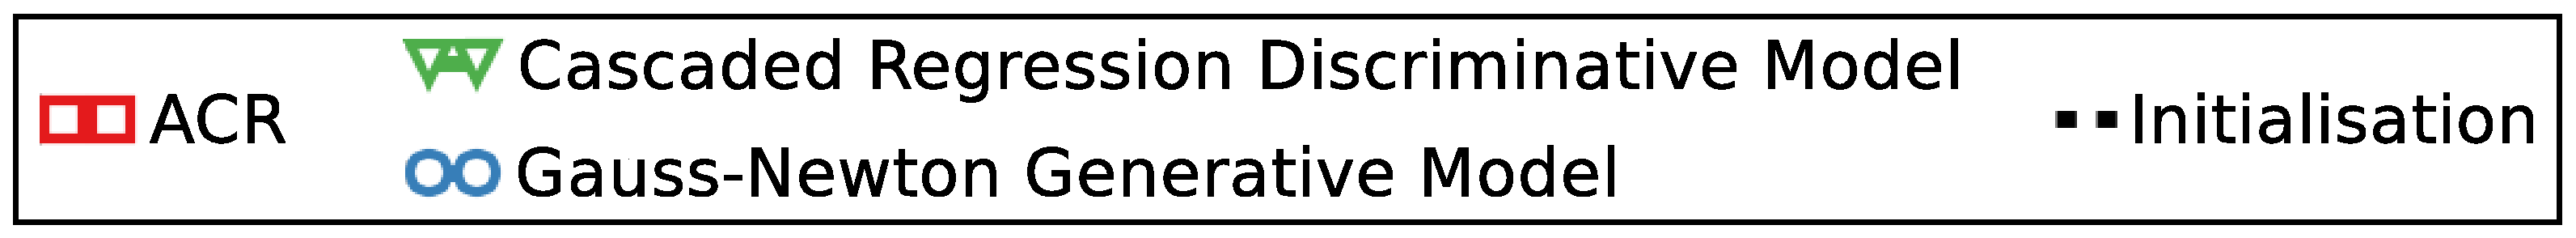
\includegraphics[height=0.90cm]{figures/acr/internal/legend/legend.eps}
  \includegraphics[width=0.70\columnwidth]{figures/acr/internal/convergence_random_runs.eps}
  \caption{Sorted initial errors of 10 random initializations of each
           image in the AFW dataset. As the initial error increases, the AAM is unable to converge, whereas ACR is both robust to initializations and consistently accurate.}
  \label{fig:self_eval_initial_errors}
\end{figure}
%%%%%%%%%%%%%%%%%%%%%%%%%%%%%%%%%%%%%%%%%%


\subsection{Self Evaluation}
In the following experiments we performed self evaluations, comparing ACR
to both the generative AAM and the discriminative SDM\@. In each case, we
trained the SDM or AAM in the same manner as the corresponding part of ACR\@.
We trained all 3 of the methods on LFPW (training, 811 images), HELEN
(training, 2000 images) and IBUG (135 images). The testing database was chosen
as AFW (337 images) as recent works (\eg,~\cite{tzimiropoulos2015project}) have
shown that AFW is still a challenging dataset.
Figure~\ref{fig:self_eval_afw_ced} shows the CED curves for the SDM, AAM and
ACR for both the 68-point and 49-point errors.
Figure~\ref{fig:self_eval_afw_ced} clearly shows the improved performance of
ACR over both SDM and AAM\@. To demonstrate the sensitivity of generative
methods to initializations, we repeated the experiment on AFW by generating 10
initializations per image and then sorted the initialization errors
(low-to-high). We then binned the initialization errors and plotted the final
error of the SDM, AAM and ACR with respect to increasing initial errors.
Figure~\ref{fig:self_eval_initial_errors} shows the results of this
initialization experiment. Here we can clearly see that, as the initialization
error increases, the AAM is incapable of converging towards an acceptable
local-minima. It also shows that, although the SDM performs well, ACR
outperforms it across all initialization errors.

\subsection{Comparison with State-of-the-Art}
In this section, we compare the performance of ACR against the state-of-the-art
methods:
%%%%%%%%%%%%%
\begin{itemize}
  \item Zhou \emph{et al.} (300W 1)~\cite{zhou2013extensive}
  \item Yan \emph{et al.} (300W 2)~\cite{yan2013learn}
  \item Coarse-to-fine Shape Searching (CFSS)~\cite{zhu2015face}
  \item Project-Out Cascaded Regression (PO-CR)~\cite{tzimiropoulos2015project}
  \item Ensemble of Regression Trees (ERT)~\cite{kazemi2014one}
  \item Intraface~\cite{xiong2013supervised,intraface2015torre}
  \item Chehra~\cite{asthana2014incremental}
\end{itemize}
%%%%%%%%%%%%%
ACR was trained using LFPW (training), HELEN (training), AFW and IBUG and both
testing and training were initialized using the bounding boxes provided by
300-W~\cite{sagonas2013300,sagonas2013300,sagonas2016faces}. The public
implementations of some of these methods only return 49-points, and
thus they are not included in the 68-point error results. We perform this
experiment on the 300-W~\cite{sagonas2013300,sagonas2013300,sagonas2016faces}
(Sec.~\ref{subsec:acr:300w}), LFPW testset~\cite{belhumeur2011localizing}
(Sec.~\ref{subsec:acr:lfpw}) and HELEN testset~\cite{le2012interactive}
(Sec.~\ref{subsec:acr:helen}) databases.

%%%%%%%%%%%%%%%%%%%%%%%%%%%%%%
%%%%%%%%%% 300 - W %%%%%%%%%%%
%%%%%%%%%%%%%%%%%%%%%%%%%%%%%%
\subsubsection{300-W Database}\label{subsec:acr:300w}
The 300-W face alignment
challenge~\cite{sagonas2013300,sagonas2013300,sagonas2016faces} utilizes a
dataset of testing images to perform evaluations. The dataset includes 600
``in-the-wild'' testing images and that are drawn from the same distribution as
the IBUG dataset. In Figure~\ref{fig:state_of_the_art}, we see that the
recently proposed CFSS method is currently the best performing method for
68-points. However, for the 49-points, ACR is the most accurate technique and
slightly outperforms (300W 1), which is a much more complex deep learning
method provided by industry. Table~\ref{tab:state_of_the_art} reinforces the
results of Figure~\ref{fig:state_of_the_art} by showing that ACR is highly
accurate for the 49-points and slightly less robust than the method
of~\cite{zhou2013extensive} over all images.

%%%%%%%%%%%%%%%%%%%%%%%%%%%%%%%%%%%%%%%%%%
\begin{figure}[!t]
  \centering
  \includegraphics[height=0.90cm]{figures/acr/state-of-the-art/legend/legend.eps}\\
  \subfloat[68-point error]{
  \includegraphics[width=0.70\linewidth]{figures/acr/state-of-the-art/68_points.eps}}\\
  \subfloat[49-point error]{
  \includegraphics[width=0.70\linewidth]{figures/acr/state-of-the-art/49_points.eps}}
  \caption{Normalized error for the testing dataset of 300-W challenge~\cite{sagonas2013300,sagonas2016faces}. This database represents a fair benchmark for state-of-the-art face alignment methods.}
  \label{fig:state_of_the_art}
\end{figure}
%%%%%%%%%%%%%%%%%%%%%%%%%%%%%%%%%%%%%%%%%%

%%%%%%%%%%%%%%%%%%%%%%%%%%%%%%%%%%%%%%%%%%
\begin{table}[!t]
  \renewcommand{\arraystretch}{1.3}
  \centering
  \begin{tabular}{|c||c|c|}
      \hline
      \emph{Method} & \emph{AUC} & \emph{Failure rate (\%)}\\
      \hline\hline
      \textbf{ACR} & \textbf{0.43} & 11.0\\\hline
      300W 1~\cite{zhou2013extensive} & 0.42 & \textbf{9.3}\\\hline
      CFSS~\cite{zhu2015face} & 0.40 & 13.5\\\hline
      300W 2~\cite{yan2013learn} & 0.38 & 14.2\\\hline
      PO-CR~\cite{tzimiropoulos2015project} & 0.37 & 17.7\\\hline
      ERT~\cite{kazemi2014one} & 0.28 & 23.7\\\hline
      Intraface~\cite{xiong2013supervised,intraface2015torre} & 0.27 & 23.8\\\hline
      Chehra~\cite{asthana2014incremental} & 0.24 & 46.8\\\hline
      Initialisation & 0.01 & 96.8\\\hline
  \end{tabular}
  \caption{The area under the curve (AUC) and percentage failure rate for the
           49-point CED curve given in Figure~\ref{fig:state_of_the_art}. Failure rate is the $\%$ of images with error~$>0.06$.}
  \label{tab:state_of_the_art}
\end{table}
%%%%%%%%%%%%%%%%%%%%%%%%%%%%%%%%%%%%%%%%%%


%%%%%%%%%%%%%%%%%%%%%%%%%%%%%%%%%%%%%%%%%%%%%%%%%
%%% LFPW
%%%%%%%%%%%%%%%%%%%%%%%%%%%%%%%%%%%%%%%%%%%%%%%%%
\subsubsection{LFPW Testset}\label{subsec:acr:lfpw}
Figure~\ref{fig:lfpw_accuracy} shows the accuracy of each method on LFPW
testset~\cite{belhumeur2013localizing} in the form of a Cumulative Error
Distribution (CED) curve. Table~\ref{tab:lfpw_accuracy} reports some
statistical measures (mean, standard deviation, median, median absolute
deviation, max), the area under the curve (AUC) and the failure rate of all
methods based on Fig.~\ref{fig:lfpw_accuracy}. Note that ACR is more accurate
than all the other methods by a large margin. Especially in the band of low
errors, it achieves an improvement of even about $10\%$. ACR is also slightly
less robust than CFSS. Another interesting observation is the very high maximum
errors for all the cascaded regression methods (PO-CR, Chehra, Intraface) that
indicate that in case of a fitting failure, the final shape is completely
scrambled.
%
\begin{figure}[!t]
  \centering
  \hspace{0.5cm}\includegraphics[height=0.90cm]{figures/acr/legend/legend.eps}\\
  \includegraphics[width=0.70\columnwidth]{figures/acr/lfpw/49_points.eps}
  \caption{Normalized error for the testing LFPW dataset based on 49 points.}
  \label{fig:lfpw_accuracy}
\end{figure}
%

%
\begin{figure}
  \centering
  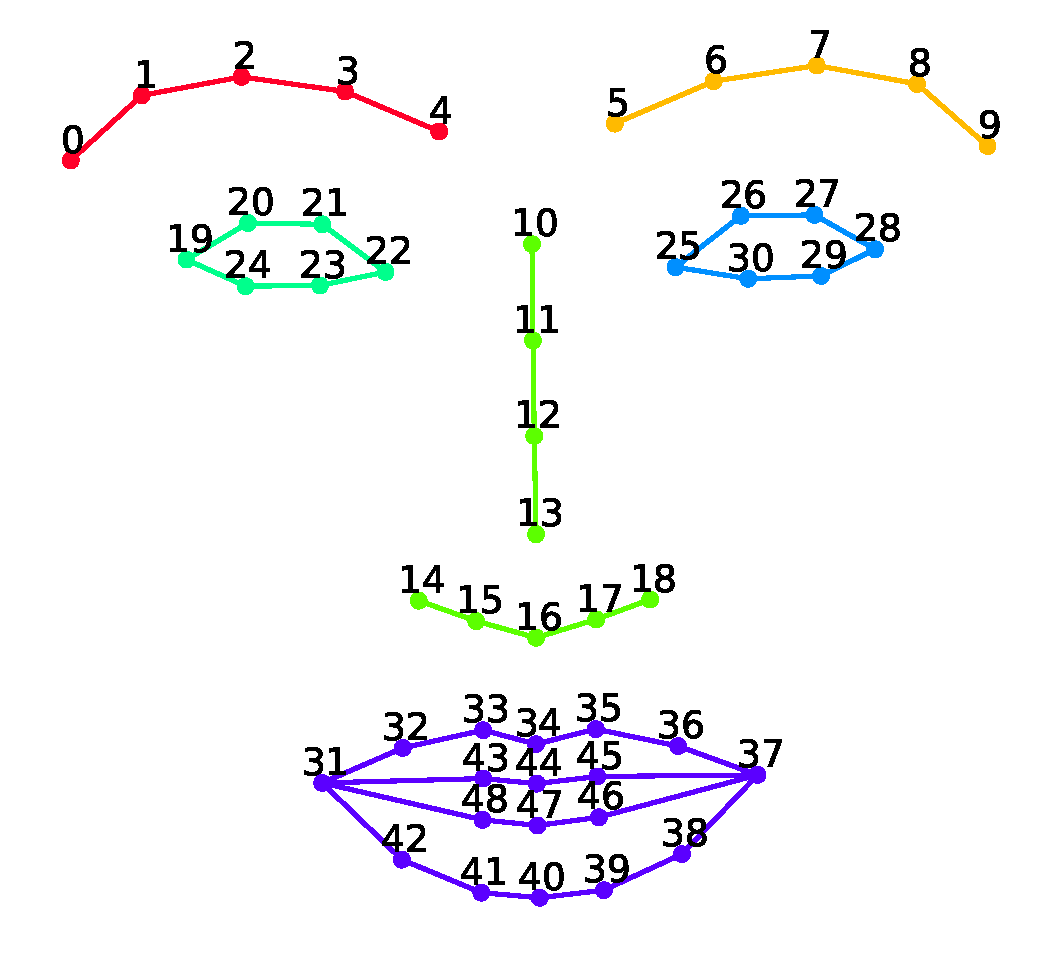
\includegraphics[width=0.5\columnwidth]{figures/acr/lfpw/mean_shape.eps}
  \caption{The numbering and grouping of the landmarks in the 49-points configuration. The coloring and numbering of this figure is to be linked with Figures~\ref{fig:lfpw_per_point} and~\ref{fig:helen_per_point}.}
\label{fig:mean_shape}
\end{figure}
%

%
\begin{table}[!t]
  \renewcommand{\arraystretch}{1.3}
  \centering
  \begin{tabular}{|c||c|c|c|c||c|c|}
      \hline
      \emph{Method} & \emph{mean $\pm$ std} & \emph{median} & \emph{mad} & \emph{max} & \emph{AUC} & \emph{Failure rate (\%)}\\
      \hline\hline
      \textbf{ACR}                                            & $\mathbf{0.0267 \pm 0.0092}$ & $\mathbf{0.0248}$ & $\mathbf{0.0045}$ & $0.0841$ & $\mathbf{0.60}$ & $1.3$\\\hline
      CFSS~\cite{zhu2015face}                                 & $0.0283 \pm 0.0079$ & $0.0270$ & $0.0046$ & $\mathbf{0.0688}$ & $0.58$ & $\mathbf{0.4}$\\\hline
      PO-CR~\cite{tzimiropoulos2015project}                   & $0.0386 \pm 0.0790$ & $0.0279$ & $0.0046$ & $0.8041$ & $0.56$ & $2.2$\\\hline
      ERT~\cite{kazemi2014one}                                & $0.0353 \pm 0.0147$ & $0.0318$ & $0.0060$ & $0.1238$ & $0.48$ & $4.0$\\\hline
      Intraface~\cite{xiong2013supervised,intraface2015torre} & $0.0666 \pm 0.1071$ & $0.0314$ & $0.0050$ & $0.6062$ & $0.46$ & $13.4$\\\hline
      Chehra~\cite{asthana2014incremental}                    & $0.0761 \pm 0.1185$ & $0.0284$ & $0.0080$ & $0.7344$ & $0.44$ & $23.7$\\\hline
      Initialisation                                          & $0.1749 \pm 0.1098$ & $0.1449$ & $0.0593$ & $0.7273$ & $0.01$ & $94.2$\\\hline
  \end{tabular}
  \caption{Various statistical measures, area under the curve (AUC) and percentage failure rate for the 49-point CED curve given in Figure~\ref{fig:lfpw_accuracy} for LFPW testset. Failure rate is the $\%$ of images with error~$>0.06$.}
  \label{tab:lfpw_accuracy}
\end{table}
%

%
\begin{figure}[!t]
  \centering
  \includegraphics[width=0.91\textwidth]{figures/acr/lfpw/ACR_per_point.eps}
  \includegraphics[width=0.91\textwidth]{figures/acr/lfpw/CFSS_per_point.eps}
  \includegraphics[width=0.91\textwidth]{figures/acr/lfpw/PO-CR_per_point.eps}
  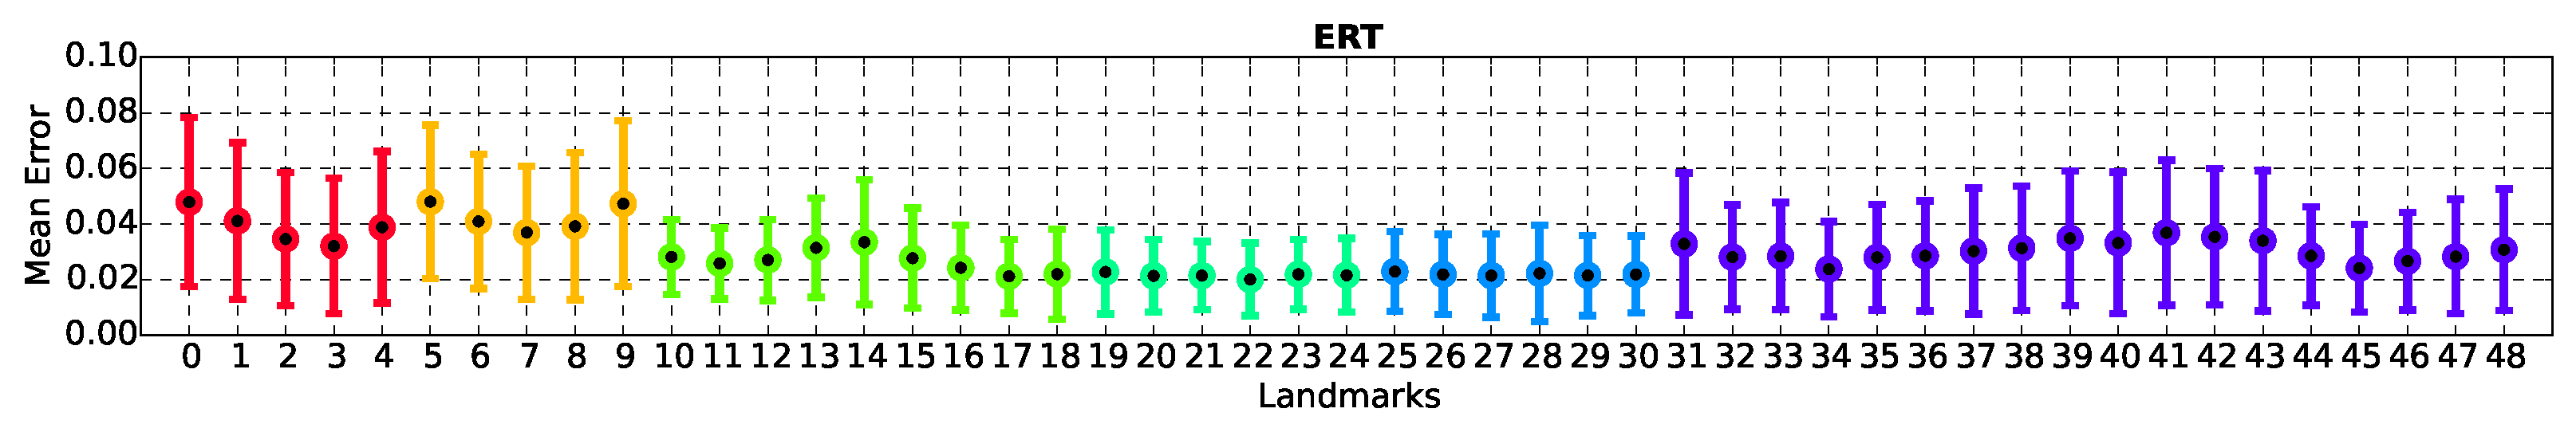
\includegraphics[width=0.91\textwidth]{figures/acr/lfpw/ERT_per_point.eps}
  \includegraphics[width=0.91\textwidth]{figures/acr/lfpw/Intraface_per_point.eps}
  \includegraphics[width=0.91\textwidth]{figures/acr/lfpw/Chehra_per_point.eps}
  \caption{Mean and standard deviation of the normalized error per landmark point for all the methods on LFPW testset. The coloring and numbering of the landmarks is linked with the mean shape of Figure~\ref{fig:mean_shape}.}
  \label{fig:lfpw_per_point}
\end{figure}
%

%
\begin{figure}[!t]
  \centering
  {
  \captionsetup[subfigure]{labelformat=empty}
  \subfloat[0.0154]{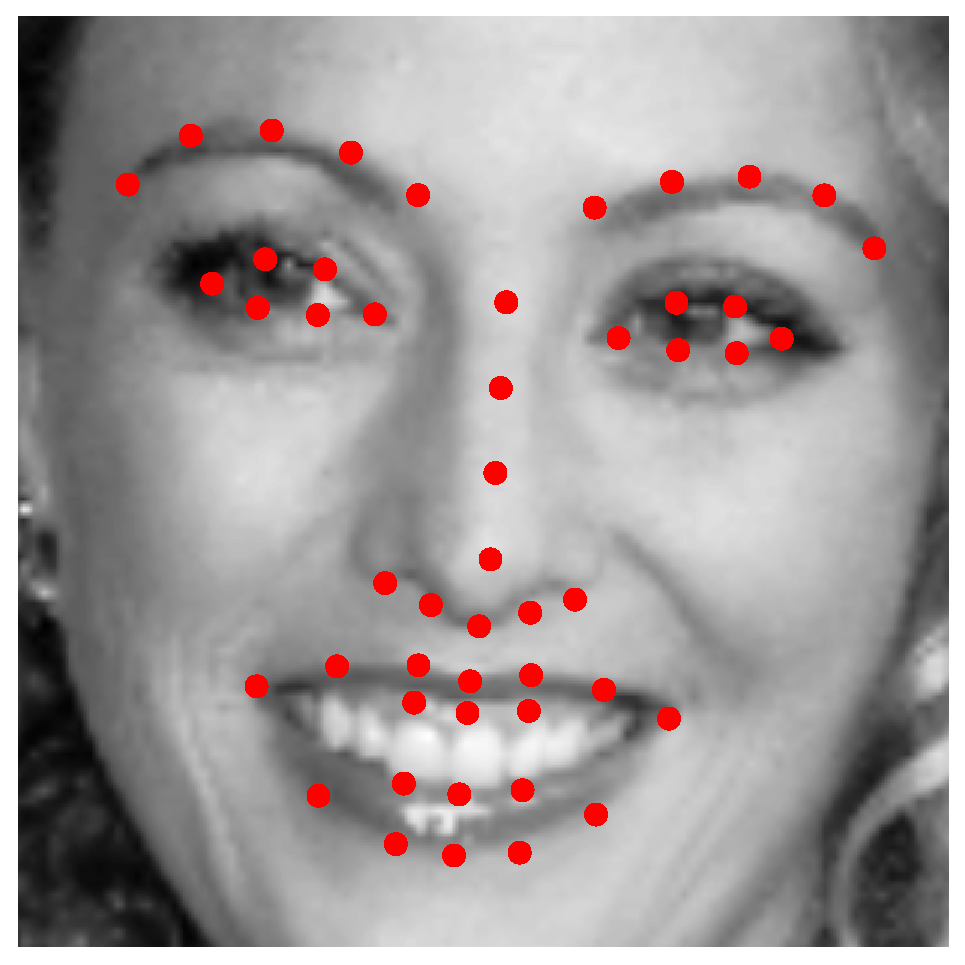
\includegraphics[width=0.1\textwidth]{figures/acr/lfpw/best/im0_err154.eps}}
  \subfloat[0.0154]{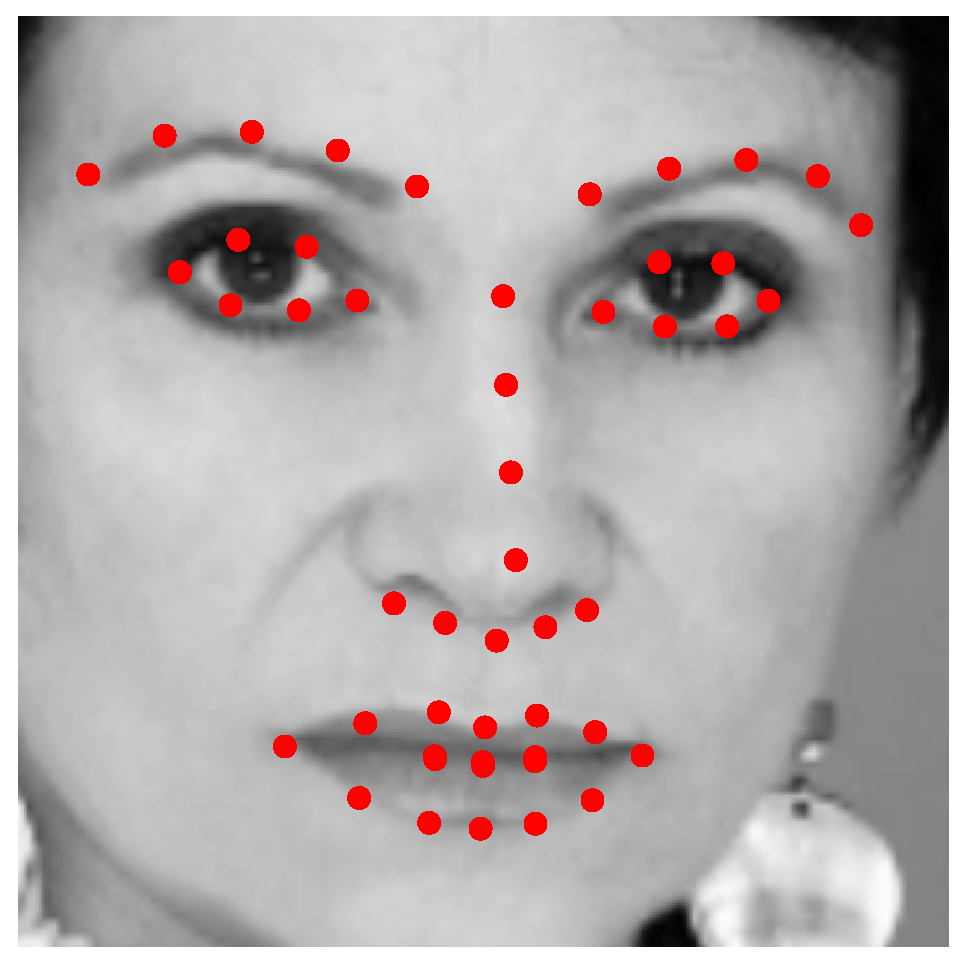
\includegraphics[width=0.1\textwidth]{figures/acr/lfpw/best/im1_err154.eps}}
  \subfloat[0.0156]{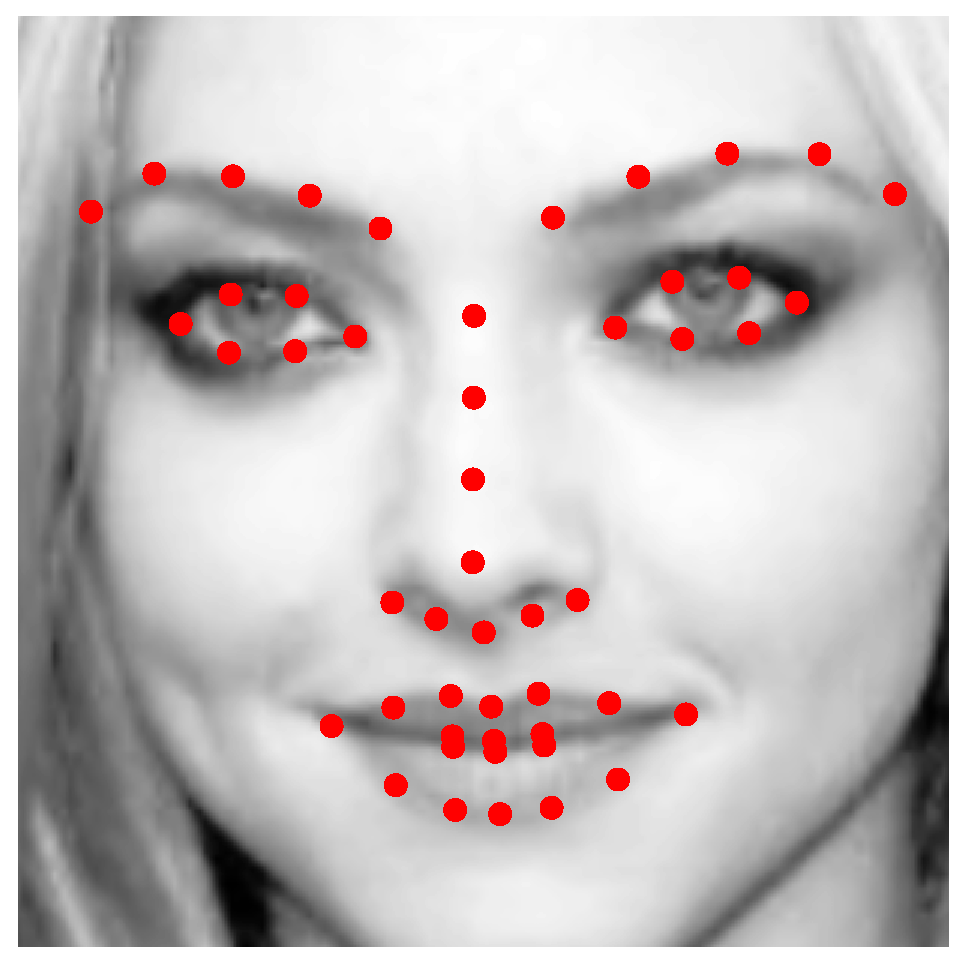
\includegraphics[width=0.1\textwidth]{figures/acr/lfpw/best/im2_err156.eps}}
  \subfloat[0.0157]{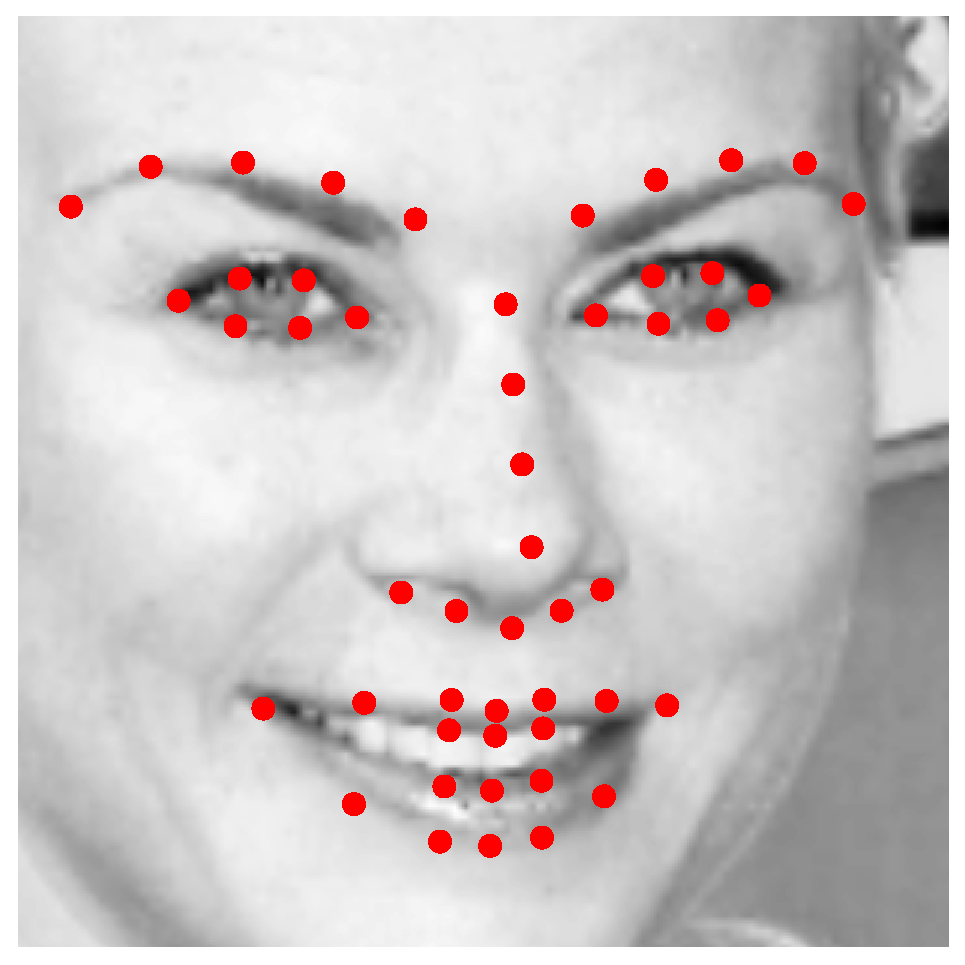
\includegraphics[width=0.1\textwidth]{figures/acr/lfpw/best/im3_err157.eps}}
  \subfloat[0.0157]{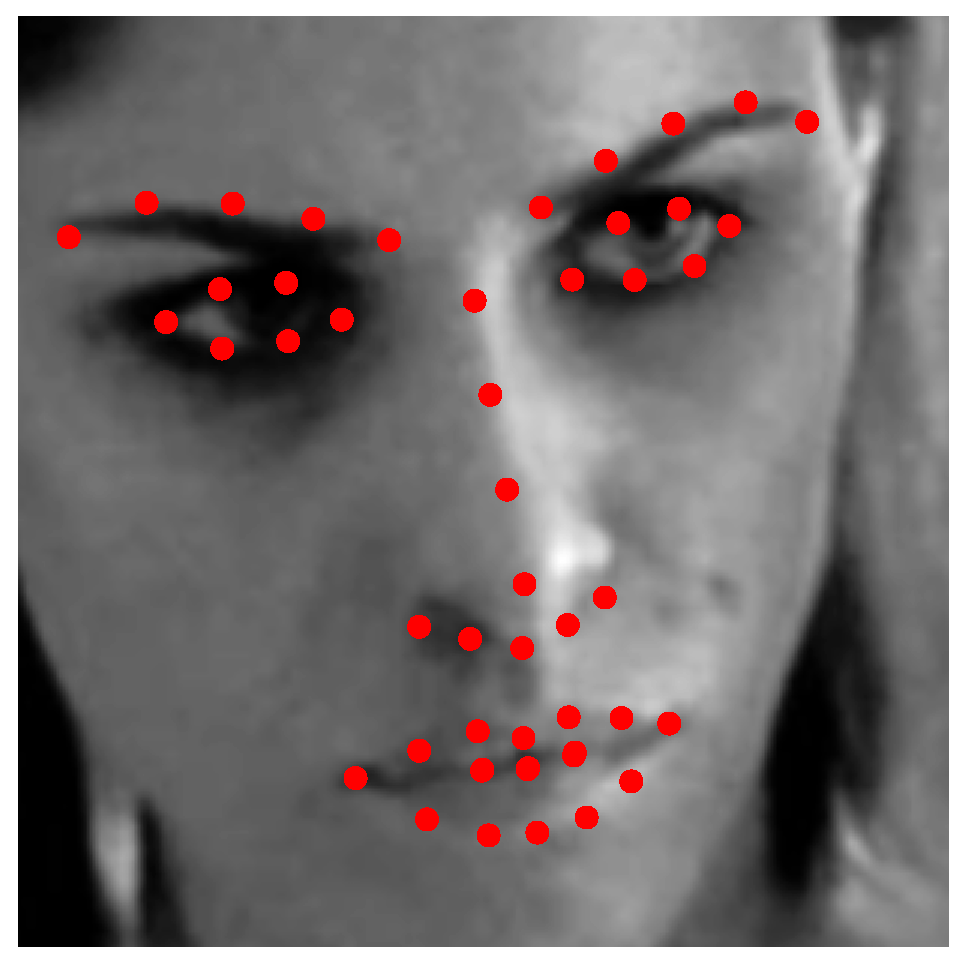
\includegraphics[width=0.1\textwidth]{figures/acr/lfpw/best/im4_err157.eps}}
  \subfloat[0.0159]{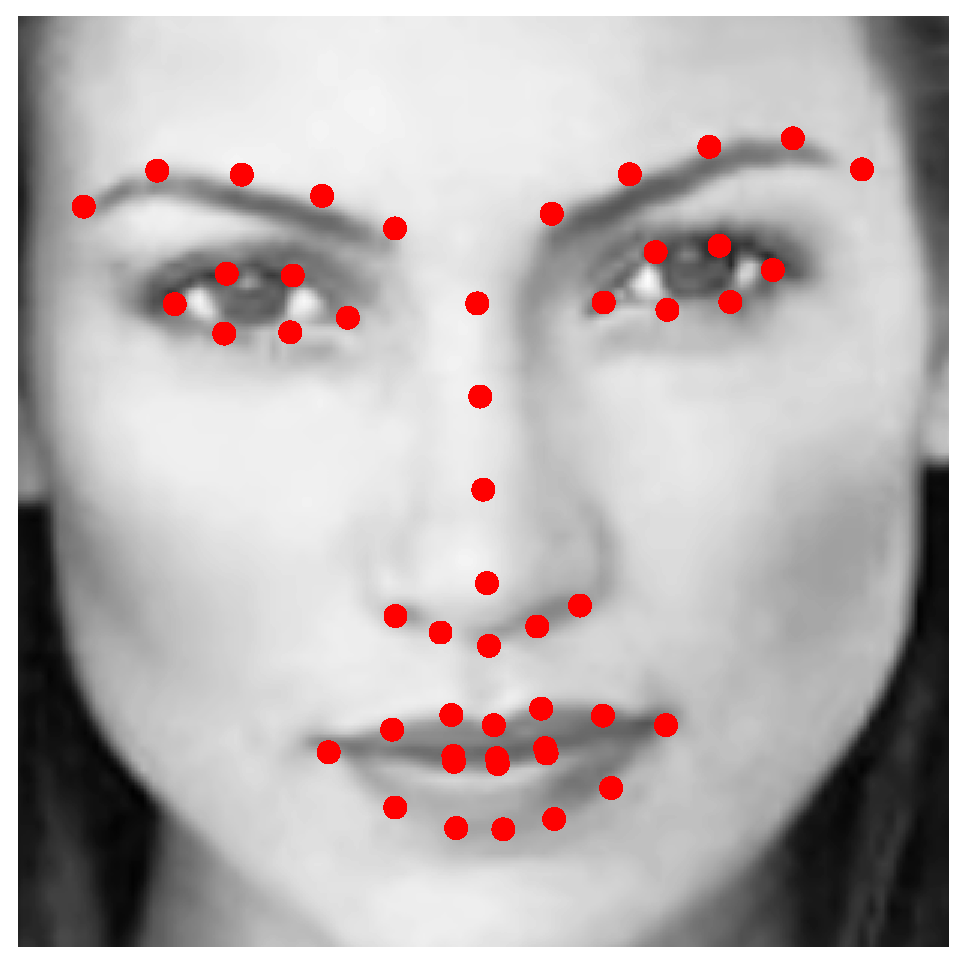
\includegraphics[width=0.1\textwidth]{figures/acr/lfpw/best/im5_err159.eps}}
  \subfloat[0.0160]{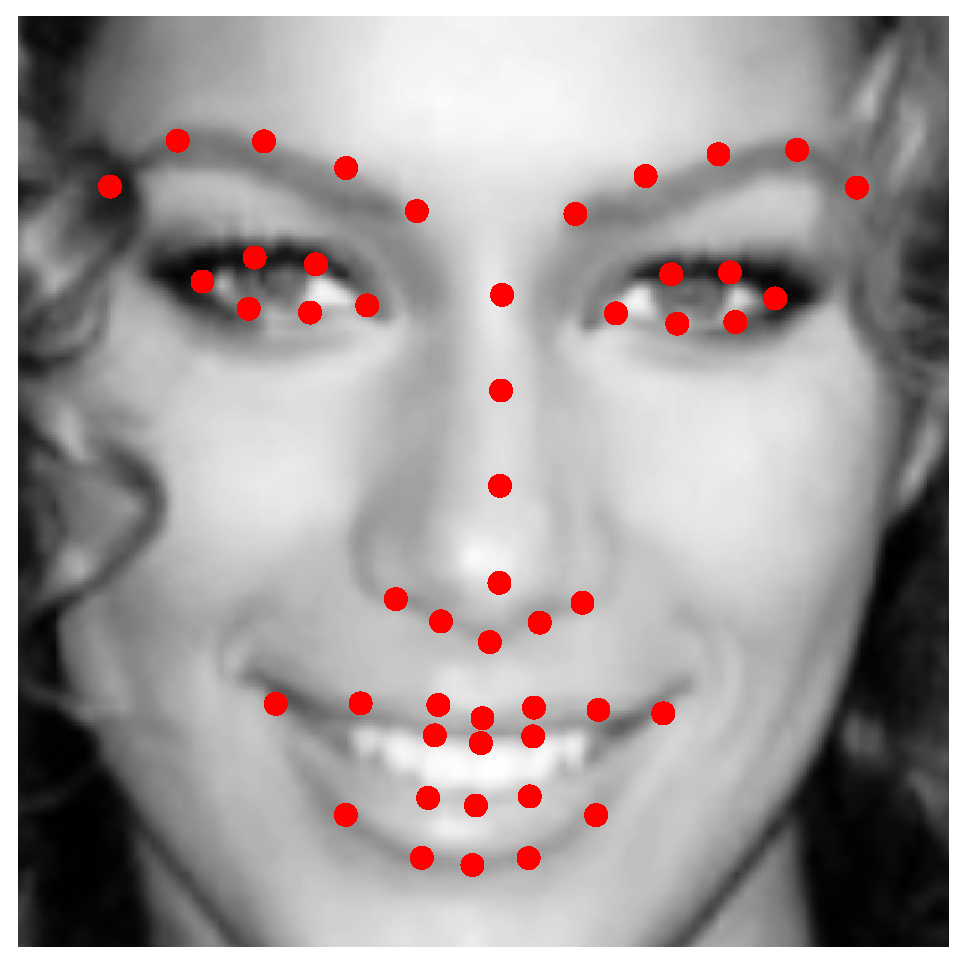
\includegraphics[width=0.1\textwidth]{figures/acr/lfpw/best/im6_err160.eps}}
  \subfloat[0.0163]{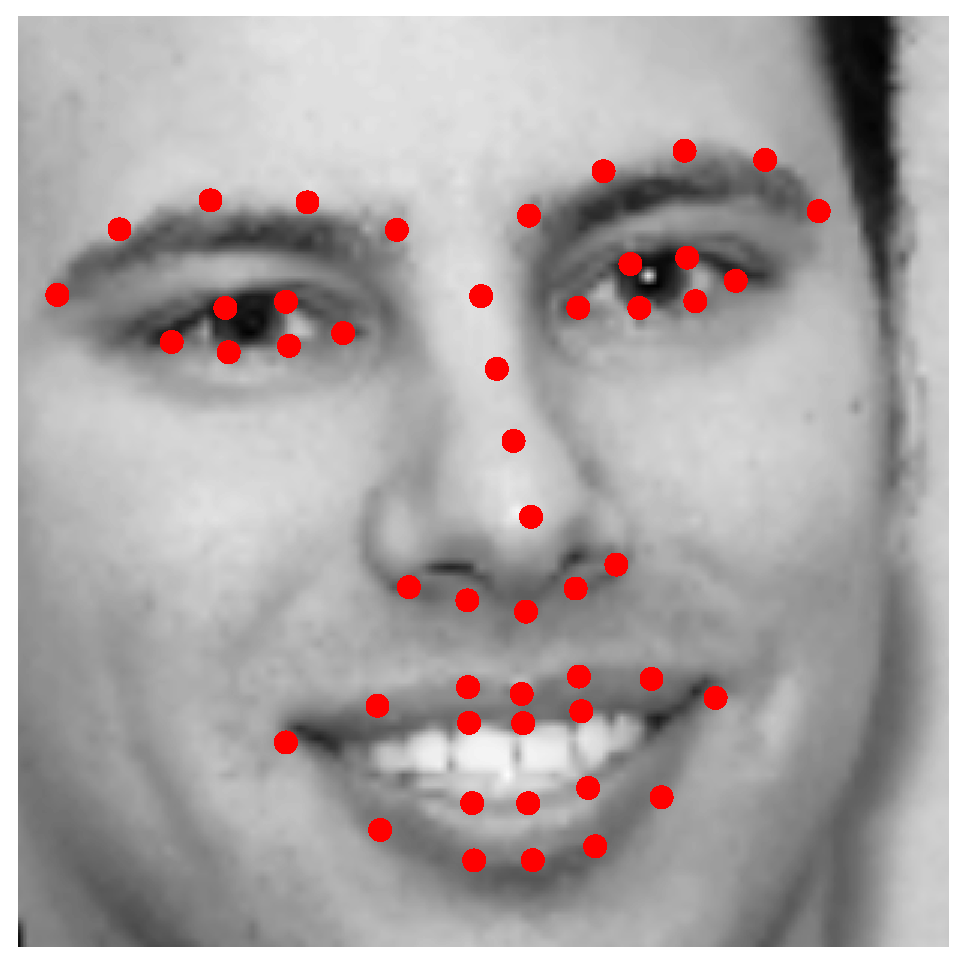
\includegraphics[width=0.1\textwidth]{figures/acr/lfpw/best/im7_err163.eps}}
  \subfloat[0.0163]{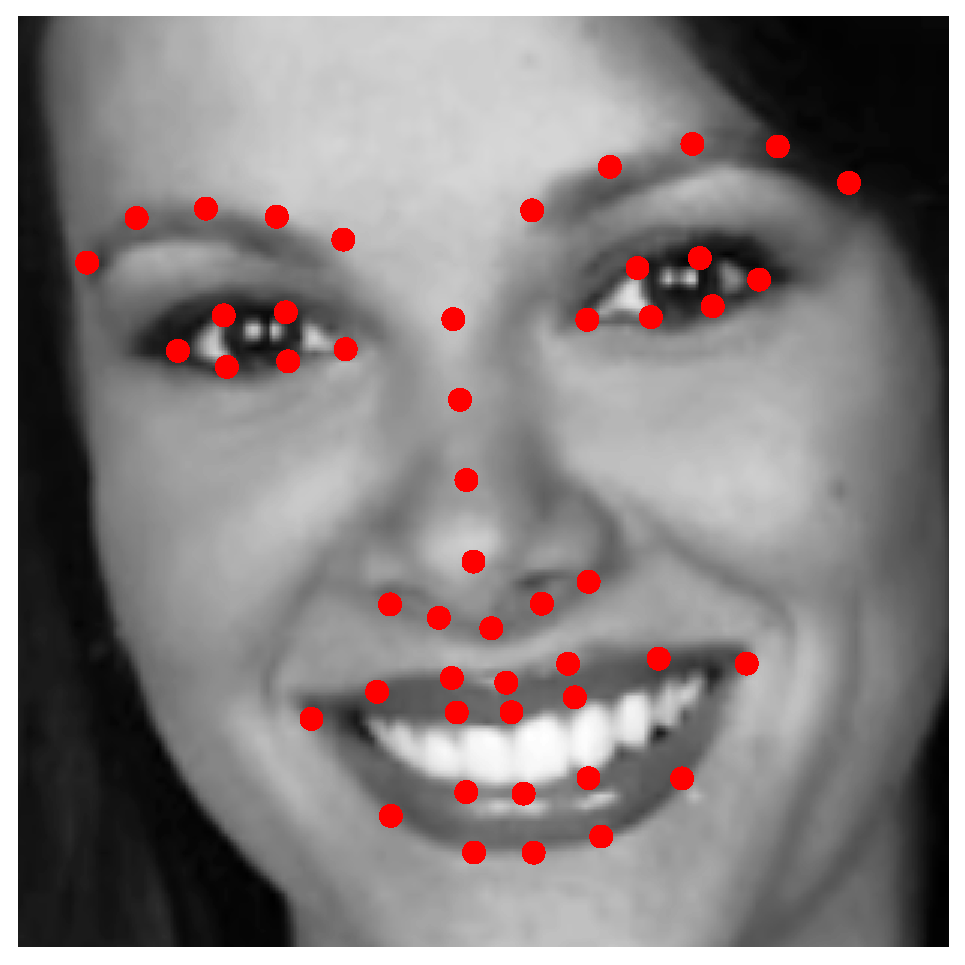
\includegraphics[width=0.1\textwidth]{figures/acr/lfpw/best/im8_err163.eps}}
  \subfloat[0.0166]{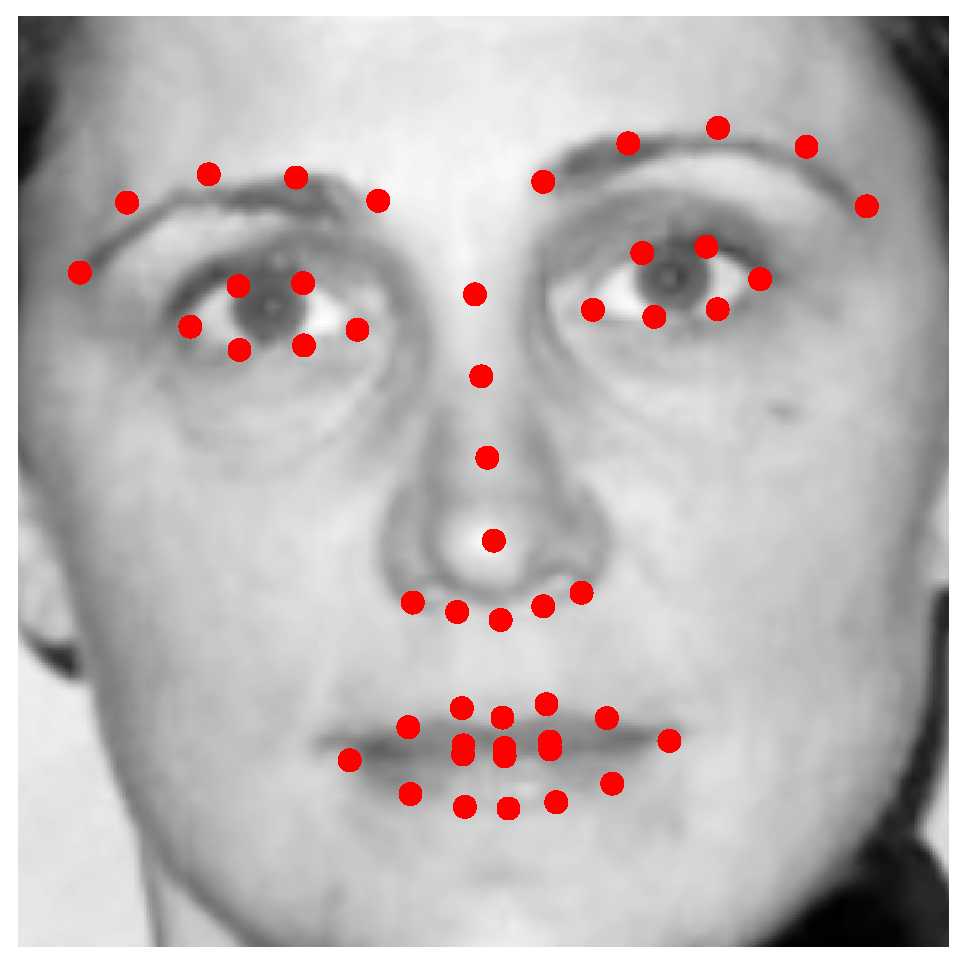
\includegraphics[width=0.1\textwidth]{figures/acr/lfpw/best/im9_err166.eps}}\\

  \subfloat[0.0418]{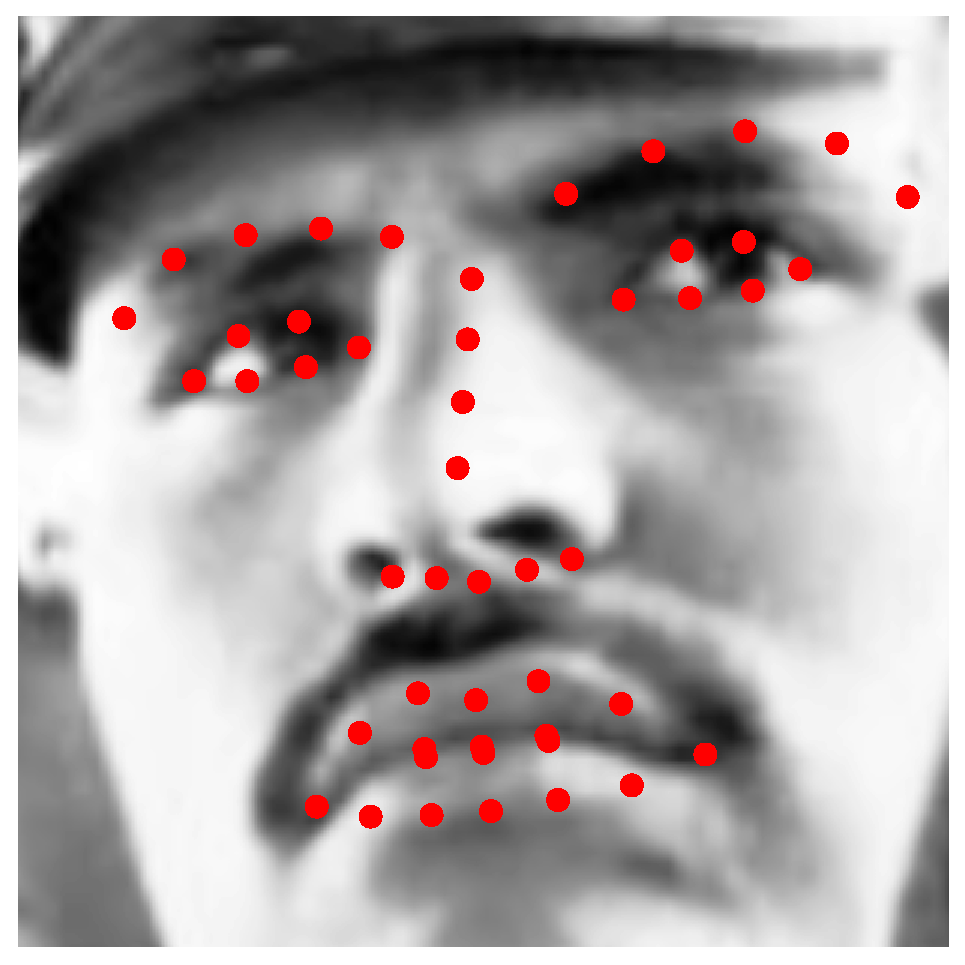
\includegraphics[width=0.1\textwidth]{figures/acr/lfpw/worst/im9_err418.eps}}
  \subfloat[0.0434]{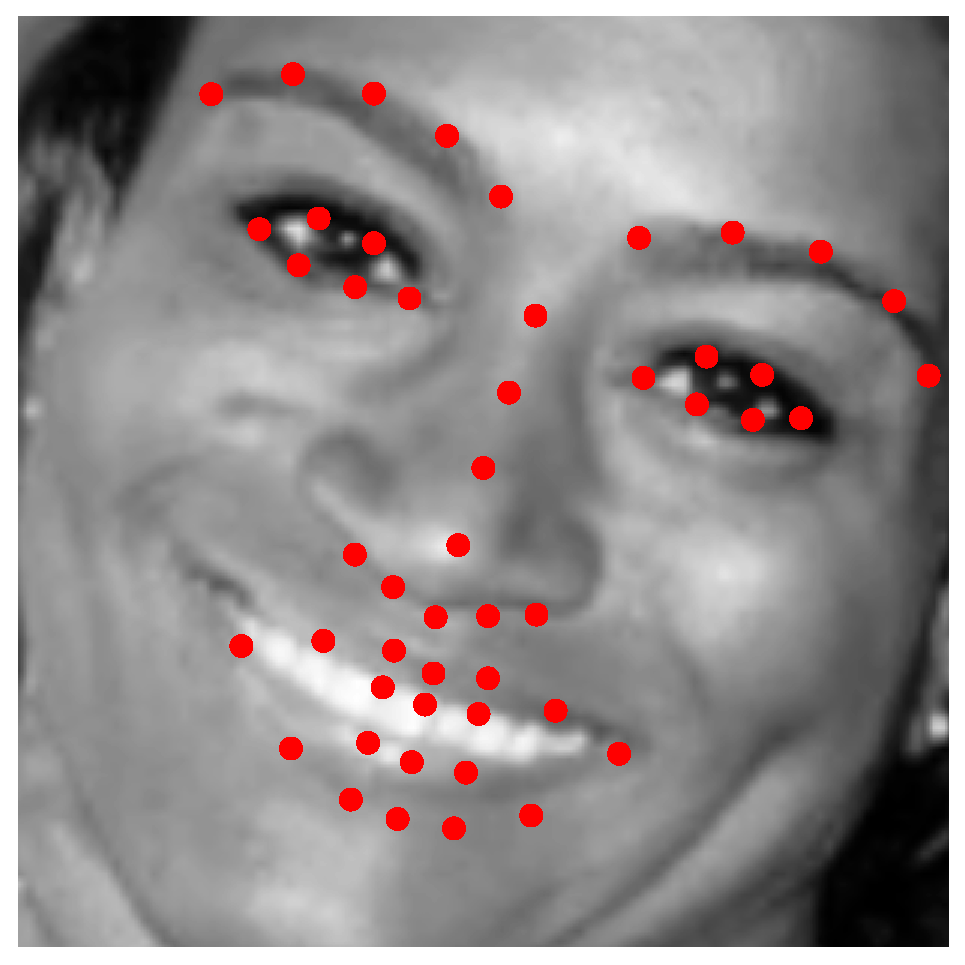
\includegraphics[width=0.1\textwidth]{figures/acr/lfpw/worst/im8_err434.eps}}
  \subfloat[0.0458]{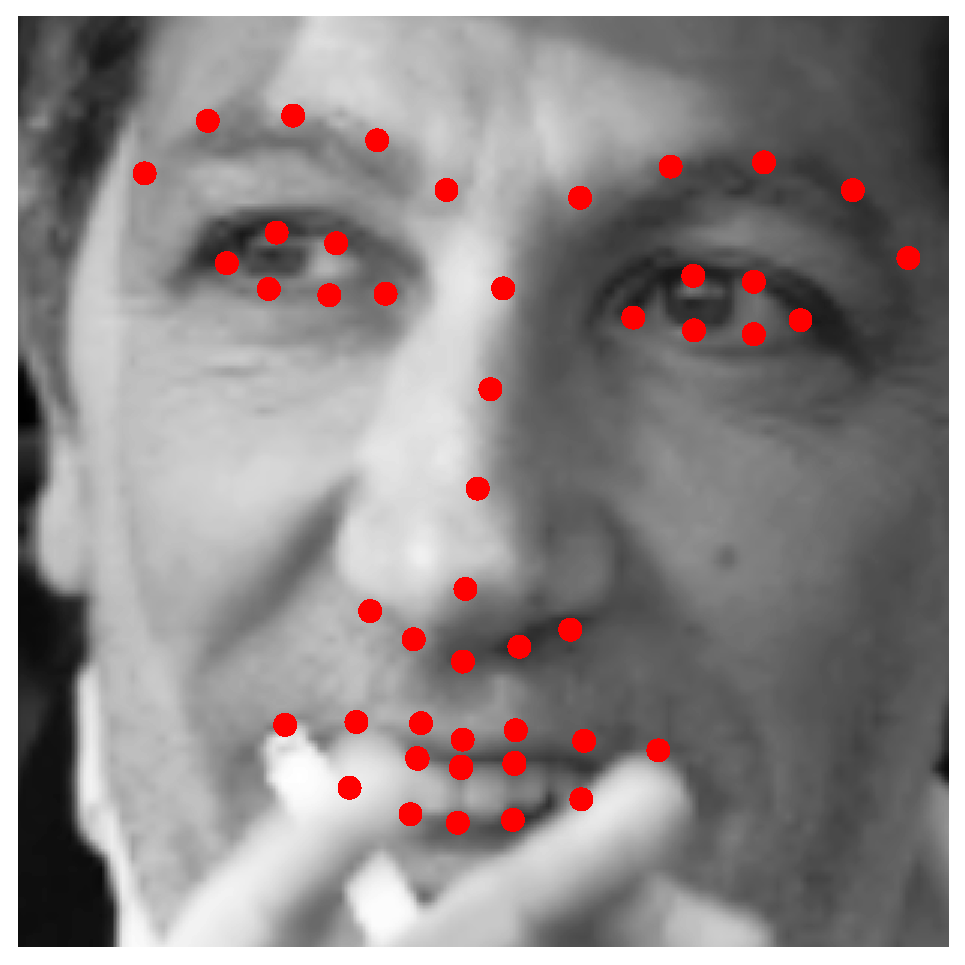
\includegraphics[width=0.1\textwidth]{figures/acr/lfpw/worst/im7_err458.eps}}
  \subfloat[0.0495]{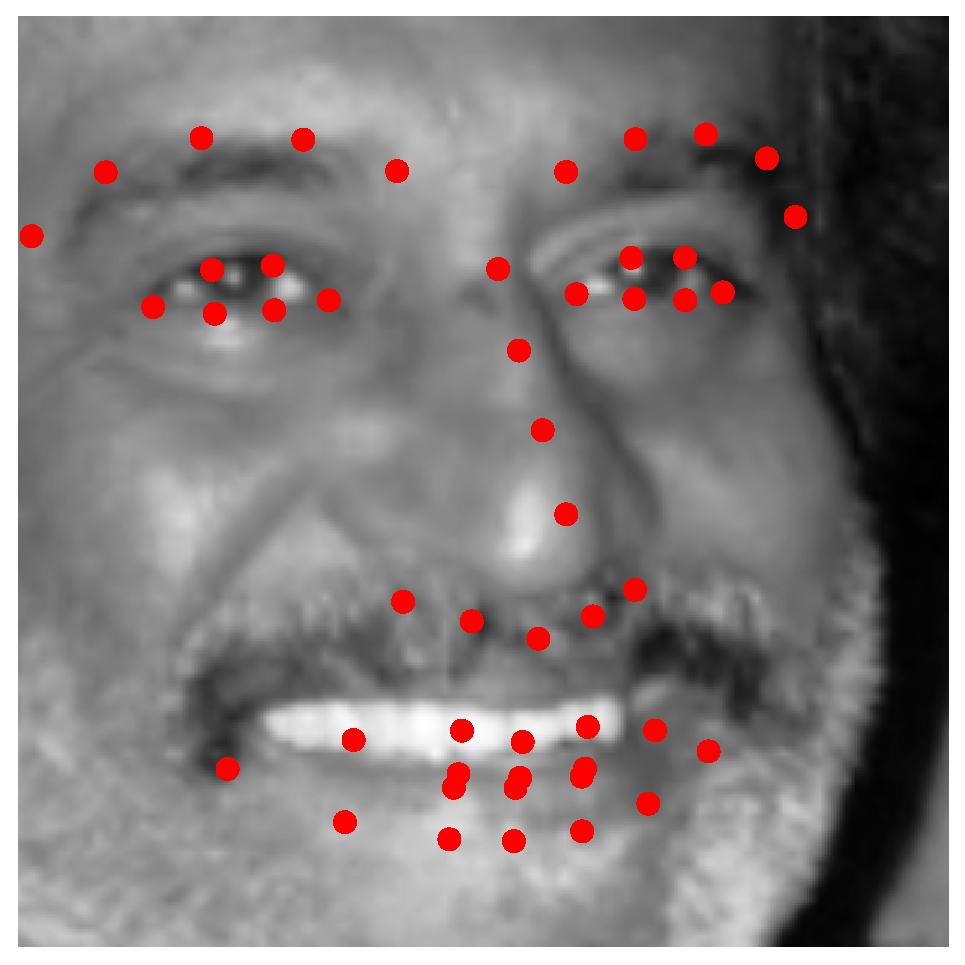
\includegraphics[width=0.1\textwidth]{figures/acr/lfpw/worst/im6_err495.eps}}
  \subfloat[0.0554]{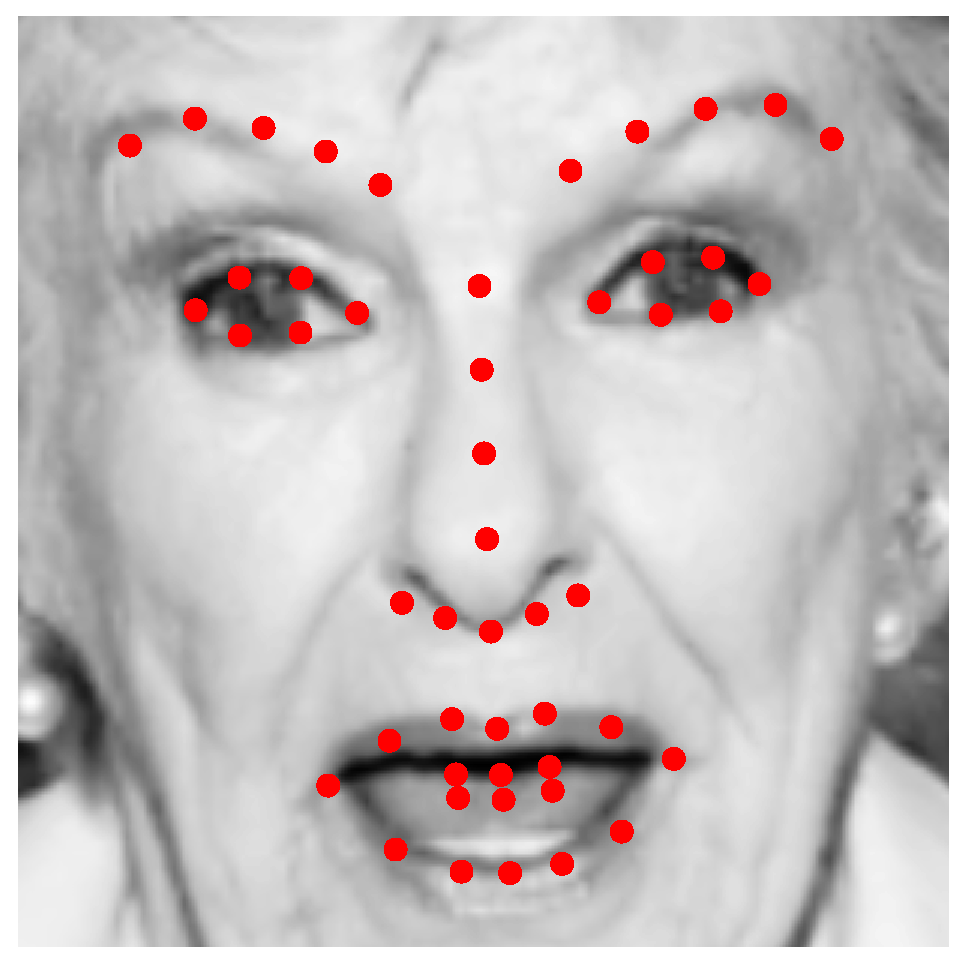
\includegraphics[width=0.1\textwidth]{figures/acr/lfpw/worst/im5_err554.eps}}
  \subfloat[0.0571]{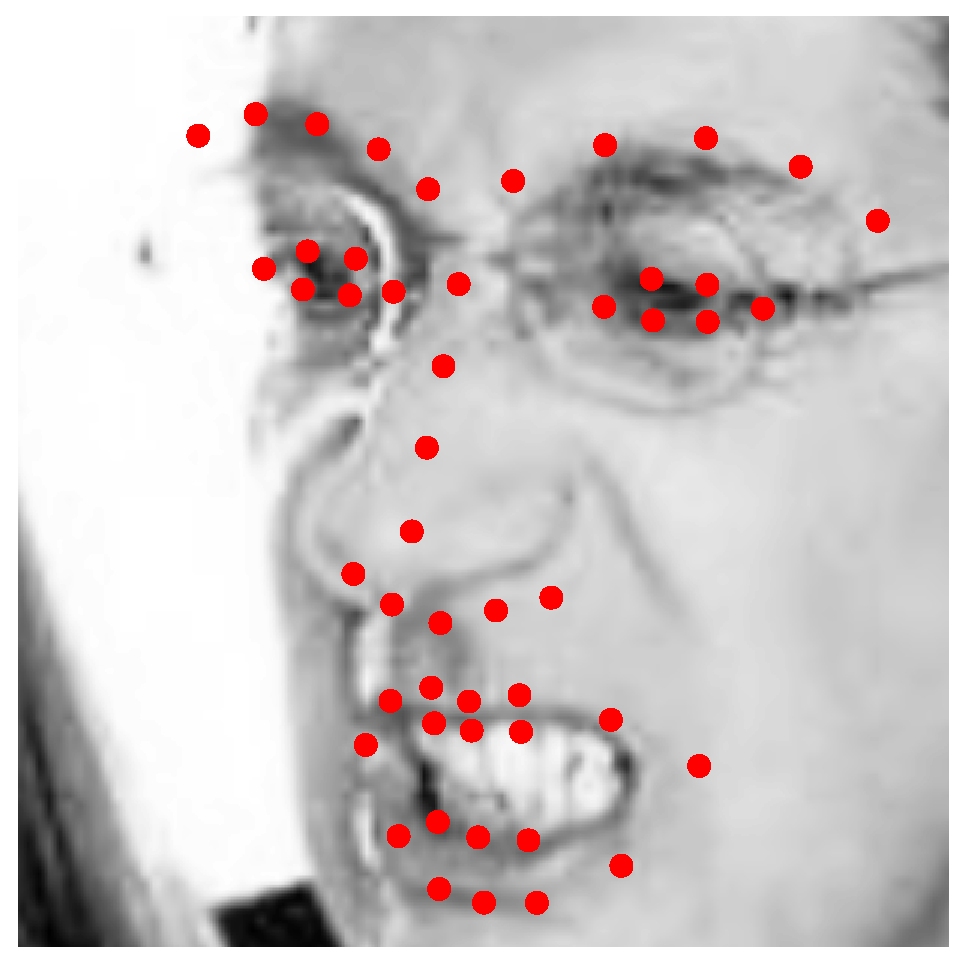
\includegraphics[width=0.1\textwidth]{figures/acr/lfpw/worst/im4_err571.eps}}
  \subfloat[0.0576]{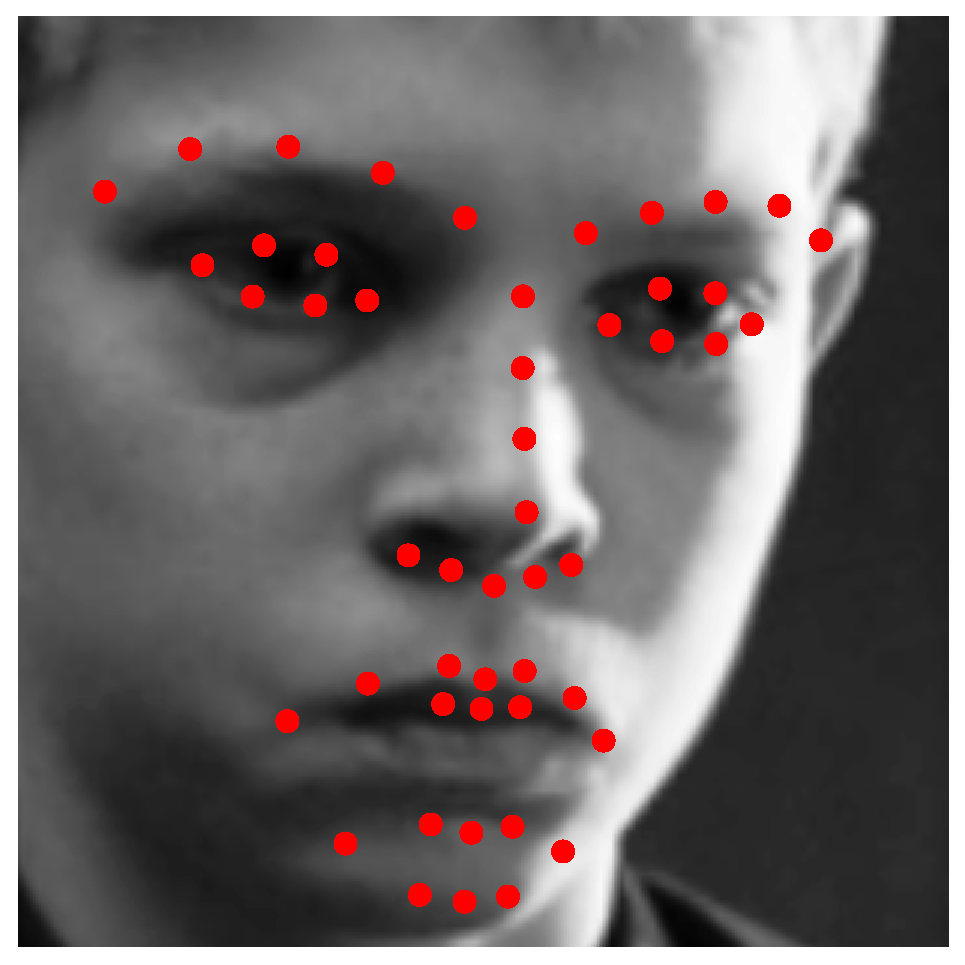
\includegraphics[width=0.1\textwidth]{figures/acr/lfpw/worst/im3_err576.eps}}
  \subfloat[0.0655]{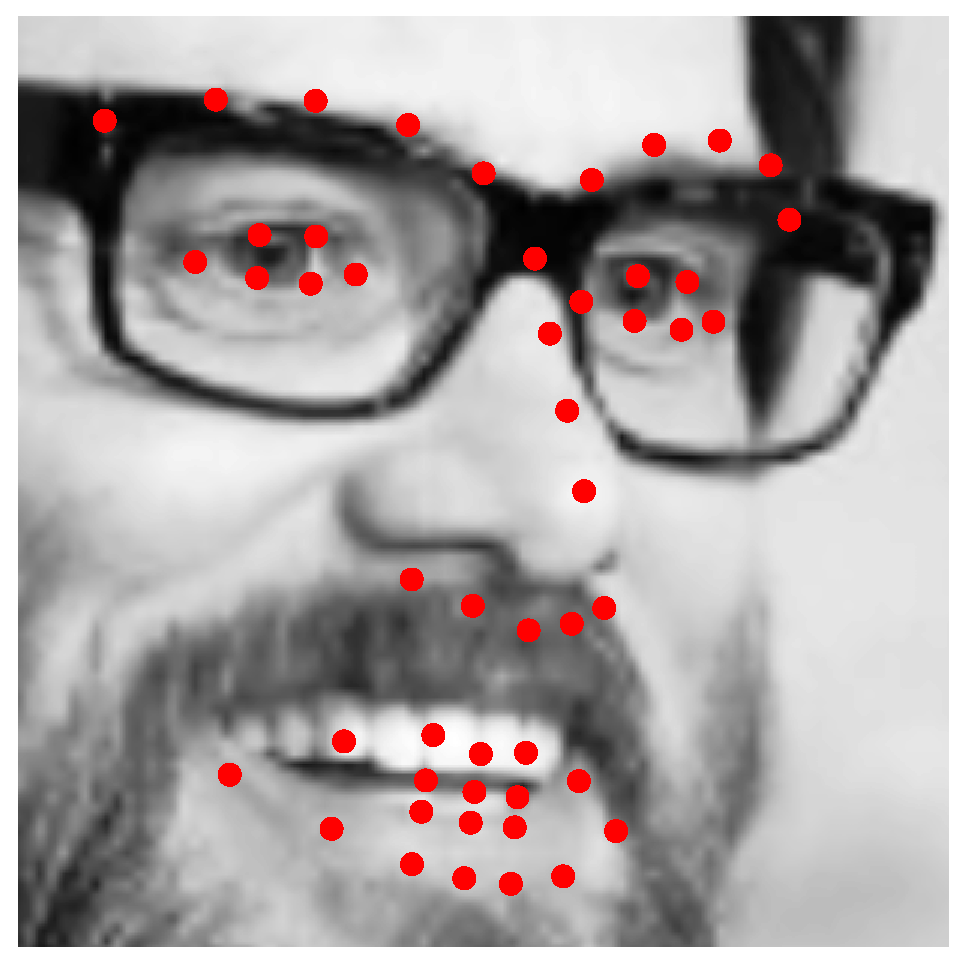
\includegraphics[width=0.1\textwidth]{figures/acr/lfpw/worst/im2_err655.eps}}
  \subfloat[0.0698]{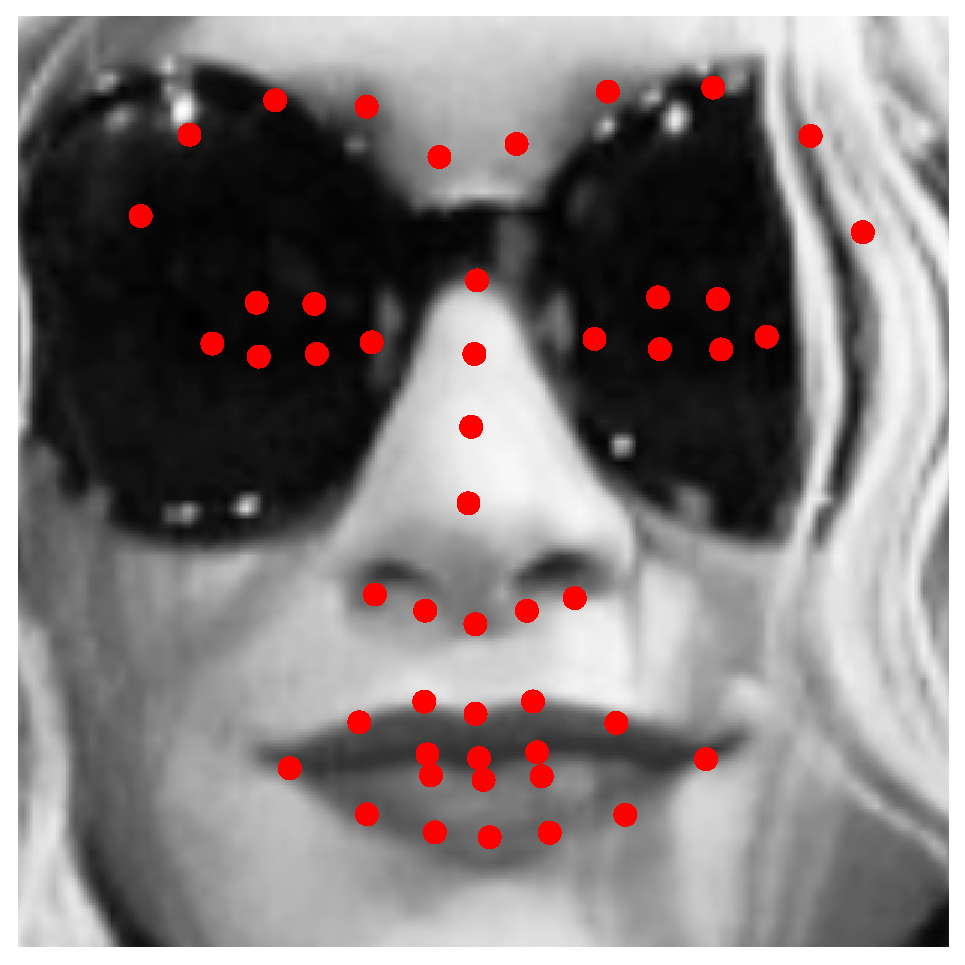
\includegraphics[width=0.1\textwidth]{figures/acr/lfpw/worst/im1_err698.eps}}
  \subfloat[0.0840]{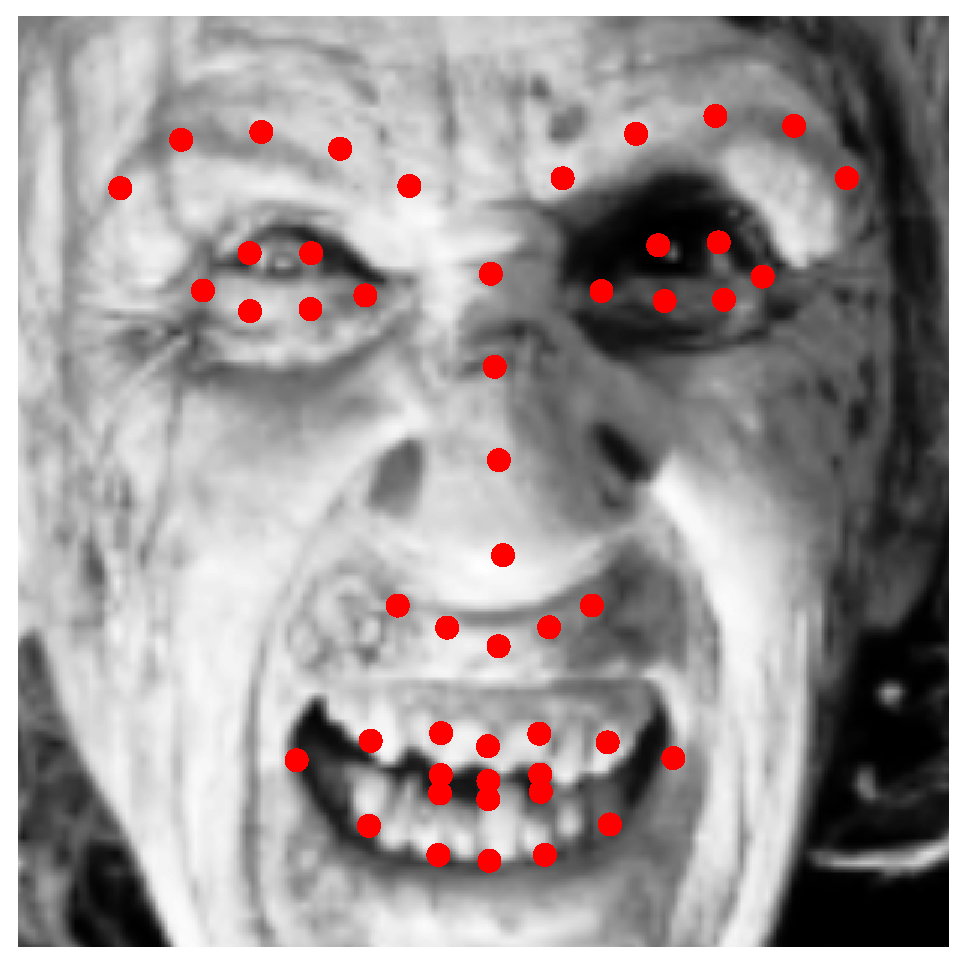
\includegraphics[width=0.1\textwidth]{figures/acr/lfpw/worst/im0_err840.eps}}
  }
  \caption{10 \emph{best} (top), and 10 \emph{worst} (bottom) fitting results of ACR on LFPW testset.}
\label{fig:lfpw_examples}
\end{figure}
%

Figure~\ref{fig:lfpw_per_point} reports the mean and standard deviation of the
error per landmark point for all the methods. The numbering and coloring of
each landmark point is linked with the mean shape of
Figure~\ref{fig:mean_shape}. Once again, note that we only take into
consideration the fittings with final error smaller than $0.06$. ACR is very
accurate on all facial parts. On the contrary, all the cascaded-regression
based techniques (PO-CR, Intraface, Chehra) heavily fail on the internal mouth
points and are not equally accurate on the eyebrows and eyes.
%
Finally, Fig.~\ref{fig:lfpw_examples} shows the 10 best and 10 worst fitting
results achieved by ACR. As it can be observed, even the worst results have not
heavily failed.


%%%%%%%%%%%%%%%%%%%%%%%%%%%%%%%%%%%%%%%%%%%%%%%%%
%%% HELEN
%%%%%%%%%%%%%%%%%%%%%%%%%%%%%%%%%%%%%%%%%%%%%%%%%
\subsubsection{HELEN Testset}\label{subsec:acr:helen}
Figure~\ref{fig:helen_accuracy} shows the accuracy of each method on the HELEN
testset~\cite{le2012interactive} in the form of a Cumulative Error Distribution
(CED) curve. Table~\ref{tab:helen_accuracy} reports some statistical measures
(mean, standard deviation, median, median absolute deviation, max), the area
under the curve (AUC) and the failure rate of all methods based on
Fig.~\ref{fig:lfpw_accuracy}. In this case, ACR is more accurate and more
robust than all the other methods, since it achieves the best AUC as well as
the lowest failure rate.

Figure~\ref{fig:helen_per_point} reports the mean and standard deviation of the
error per landmark point for all the methods. Similar to the LFPW case, the
numbering and coloring of each landmark point is linked with the mean shape of
Figure~\ref{fig:mean_shape}. The results are again similar and indicate that
ACR is more accurate on all facial parts, especially on the mouth region.
%
Finally, Fig.~\ref{fig:helen_examples} shows the 10 best and 10 worst fitting
results achieved by ACR.

%
\begin{figure}[!t]
  \centering
  \hspace{0.5cm}\includegraphics[height=0.90cm]{figures/acr/legend/legend.eps}\\
  \includegraphics[width=0.70\columnwidth]{figures/acr/helen/49_points.eps}
  \caption{Normalized error for the testing HELEN dataset based on 49 points.}
\label{fig:helen_accuracy}
\end{figure}
%

%
\begin{table}[!t]
  \renewcommand{\arraystretch}{1.3}
  \centering
  \begin{tabular}{|c||c|c|c|c||c|c|}
      \hline
      \emph{Method} & \emph{mean $\pm$ std} & \emph{median} & \emph{mad} & \emph{max} & \emph{AUC} & \emph{Failure rate (\%)}\\
      \hline\hline
      \textbf{ACR}                                            & $\mathbf{0.0262 \pm 0.0104}$ & $\mathbf{0.0240}$ & $0.0050$ & $\mathbf{0.0968}$ & $\mathbf{0.61}$ & $\mathbf{1.2}$\\\hline
      CFSS~\cite{zhu2015face}                                 & $0.0288 \pm 0.0318$ & $0.0244$ & $\mathbf{0.0048}$ & $0.5644$ & $0.60$ & $1.5$\\\hline
      PO-CR~\cite{tzimiropoulos2015project}                   & $0.0299 \pm 0.0287$ & $0.0260$ & $0.0051$ & $0.5199$ & $0.58$ & $0.6$\\\hline
      ERT~\cite{kazemi2014one}                                & $0.0323 \pm 0.0236$ & $0.0280$ & $0.0055$ & $0.3732$ & $0.54$ & $1.8$\\\hline
      Intraface~\cite{xiong2013supervised,intraface2015torre} & $0.0666 \pm 0.1094$ & $0.0336$ & $0.0060$ & $0.7718$ & $0.45$ & $11.5$\\\hline
      Chehra~\cite{asthana2014incremental}                    & $0.0391 \pm 0.0507$ & $0.0251$ & $0.0054$ & $0.4853$ & $0.55$ & $9.4$\\\hline
      Initialisation                                          & $0.1757 \pm 0.1050$ & $0.1475$ & $0.0603$ & $0.5656$ & $0.02$ & $90.9$\\\hline
  \end{tabular}
  \caption{Various statistical measures, area under the curve (AUC) and percentage failure rate for the 49-point CED curve given in Figure~\ref{fig:helen_accuracy} for HELEN testset. Failure rate is the $\%$ of images with error~$>0.06$.}
\label{tab:helen_accuracy}
\end{table}
%

%
\begin{figure}[!t]
  \centering
  \includegraphics[width=0.91\textwidth]{figures/acr/helen/ACR_per_point.eps}
  \includegraphics[width=0.91\textwidth]{figures/acr/helen/CFSS_per_point.eps}
  \includegraphics[width=0.91\textwidth]{figures/acr/helen/PO-CR_per_point.eps}
  \includegraphics[width=0.91\textwidth]{figures/acr/helen/ERT_per_point.eps}
  \includegraphics[width=0.91\textwidth]{figures/acr/helen/Intraface_per_point.eps}
  \includegraphics[width=0.91\textwidth]{figures/acr/helen/Chehra_per_point.eps}
  \caption{Mean and standard deviation of the normalized error per landmark point for all the methods on HELEN testset. The coloring and numbering of the landmarks is linked with the mean shape of Figure~\ref{fig:mean_shape}.}
\label{fig:helen_per_point}
\end{figure}
%

%
\begin{figure}[!t]
  \centering
  {
  \captionsetup[subfigure]{labelformat=empty}
  \subfloat[0.0119]{\includegraphics[width=0.1\textwidth]{figures/acr/helen/best/im0_err119.eps}}
  \subfloat[0.0122]{\includegraphics[width=0.1\textwidth]{figures/acr/helen/best/im1_err122.eps}}
  \subfloat[0.0124]{\includegraphics[width=0.1\textwidth]{figures/acr/helen/best/im2_err124.eps}}
  \subfloat[0.0129]{\includegraphics[width=0.1\textwidth]{figures/acr/helen/best/im3_err129.eps}}
  \subfloat[0.0133]{\includegraphics[width=0.1\textwidth]{figures/acr/helen/best/im4_err133.eps}}
  \subfloat[0.0136]{\includegraphics[width=0.1\textwidth]{figures/acr/helen/best/im6_err136.eps}}
  \subfloat[0.0144]{\includegraphics[width=0.1\textwidth]{figures/acr/helen/best/im7_err144.eps}}
  \subfloat[0.0144]{\includegraphics[width=0.1\textwidth]{figures/acr/helen/best/im8_err144.eps}}
  \subfloat[0.0145]{\includegraphics[width=0.1\textwidth]{figures/acr/helen/best/im9_err145.eps}}
  \subfloat[0.0147]{\includegraphics[width=0.1\textwidth]{figures/acr/helen/best/im10_err147.eps}}\\

  \subfloat[0.0493]{\includegraphics[width=0.1\textwidth]{figures/acr/helen/worst/im9_err493.eps}}
  \subfloat[0.0504]{\includegraphics[width=0.1\textwidth]{figures/acr/helen/worst/im8_err504.eps}}
  \subfloat[0.0518]{\includegraphics[width=0.1\textwidth]{figures/acr/helen/worst/im7_err518.eps}}
  \subfloat[0.0528]{\includegraphics[width=0.1\textwidth]{figures/acr/helen/worst/im6_err528.eps}}
  \subfloat[0.0592]{\includegraphics[width=0.1\textwidth]{figures/acr/helen/worst/im5_err592.eps}}
  \subfloat[0.0619]{\includegraphics[width=0.1\textwidth]{figures/acr/helen/worst/im4_err619.eps}}
  \subfloat[0.0666]{\includegraphics[width=0.1\textwidth]{figures/acr/helen/worst/im3_err666.eps}}
  \subfloat[0.0791]{\includegraphics[width=0.1\textwidth]{figures/acr/helen/worst/im2_err791.eps}}
  \subfloat[0.0878]{\includegraphics[width=0.1\textwidth]{figures/acr/helen/worst/im1_err878.eps}}
  \subfloat[0.0968]{\includegraphics[width=0.1\textwidth]{figures/acr/helen/worst/im0_err968.eps}}
  }
  \caption{10 \emph{best} (top), and 10 \emph{worst} (bottom) fitting results of ACR on HELEN testset.}
\label{fig:helen_examples}
\end{figure}
%
